\graphicspath{{./chapters/rt-from-frequency-dynamics/}}
\chapter{Supplementary Materials for Chapter 2} 

\section{Supplementary Text}

\subsection*{Relationship to multinomial logistic regression}

Other papers have tried to infer growth advantages of variants from sequence data alone, we show that the multinomial logistic regression model typically used in these analysis is roughly equivalent to our fixed growth advantage model, but that inferring relative effective reproduction numbers between variants using multinomial logistic regression requires additional restrictions on the generation time.
Multinomial logistic regression typically models the probability of a given observation belong to class $v$ at time $t$ as
\begin{equation}
  f_{v}(t) = \frac{p_{v}\exp(\beta_{v} t)}{\sum_{1\leq u\leq V} p_{u}\exp(\beta_{u} t)}.
\end{equation}
For our purpose, we can assume this probability is equivalent to the true frequency of variant $v$ in the population and in this case, $p_{v}$ is considered to be related to the prevalence on variant $v$ in the population at $t=0$ and $\beta_{v}$ can be considered to be the growth advantage relative to a pivot class $u_{*}$ which has $\beta_{k_{*}} = 0$.
In order to see the connection between the above model and ours, we return to the original renewal equation of the form
\begin{equation}
  I(t) = R_{t}\int_{0}^{t} I(t-\tau) g(\tau).
\end{equation}
Assuming that $g$  is a point mass at a mean generation time $T_{g}$, we have that
\begin{equation}
  I(nT_{g}) = \left(\prod_{i=1}^{n} R_{iT_{g}}\right) I(0).
\end{equation}
Assuming that there are several variants following these same dynamics, we have that the frequency of a given variant $v$ can be written as
\begin{equation}
  f_{v}(nT_{g}) = \frac{I_{v}(nT_{g})}{\sum_{1\leq u \leq V} I_{u}(nT_{g})}.
\end{equation}
If we assume a constant growth advantage as in our model, we then have that $R_{t,v} = \Delta_{v} R_{t}$, so that
\begin{equation}
  f_{v}(nT_{g}) =  \frac{\Delta_{v}^{n} I_{v}(0)}{\sum_{1\leq u \leq V} \Delta_{u}^{n} I_{u}(0)}.
\end{equation}
Writing $\Delta_{v} = \exp(\delta_{v})$ and $t = n T_{g}$, allows us to see that
\begin{equation}
  f_{v}(t) = \frac{I_{v}(0) \exp(\frac{\delta_{v}}{T_{g}} t)}{\sum_{1\leq u \leq V}I_{u}(0) \exp(\frac{\delta_{u}}{T_{g}} t)}.
\end{equation}
By fixing one pivot class so that $I_{u_{*}} = 1$ and $\delta_{u_{*}} / T_{g} = 0$, we can identify our model with the multinomial logistic regression by relating the parameters as

\begin{align}
  \delta_{v} &= \beta_{v}T_{g}\\
  I_{v}(0) &= p_{v}.
\end{align}

This shows that the multinomial logistic regression functions similarly to our fixed growth advantage model except with the additional assumption that the generation time is a point mass at $T_{g}$.
This assumption additionally allows us to relate the epidemic growth rate $r$ and the effective reproduction number as $R = \exp(r T_{g})$ \cite{Wallinga2006}.
Therefore, by further assuming that the variant infections are exponentially growing with rates $r_{v}$, we can then identify $\beta_{v} = r_{v} - r_{u_{*}}$.
This means that the relative effective reproduction number for any two variants can be written as
\begin{align*}
\ln \left( \frac{R_{t,v}}{R_{t,u}} \right) = (\beta_{v} - \beta_{u}) T_{g}.
\end{align*}

\begin{figure}
  \centering
  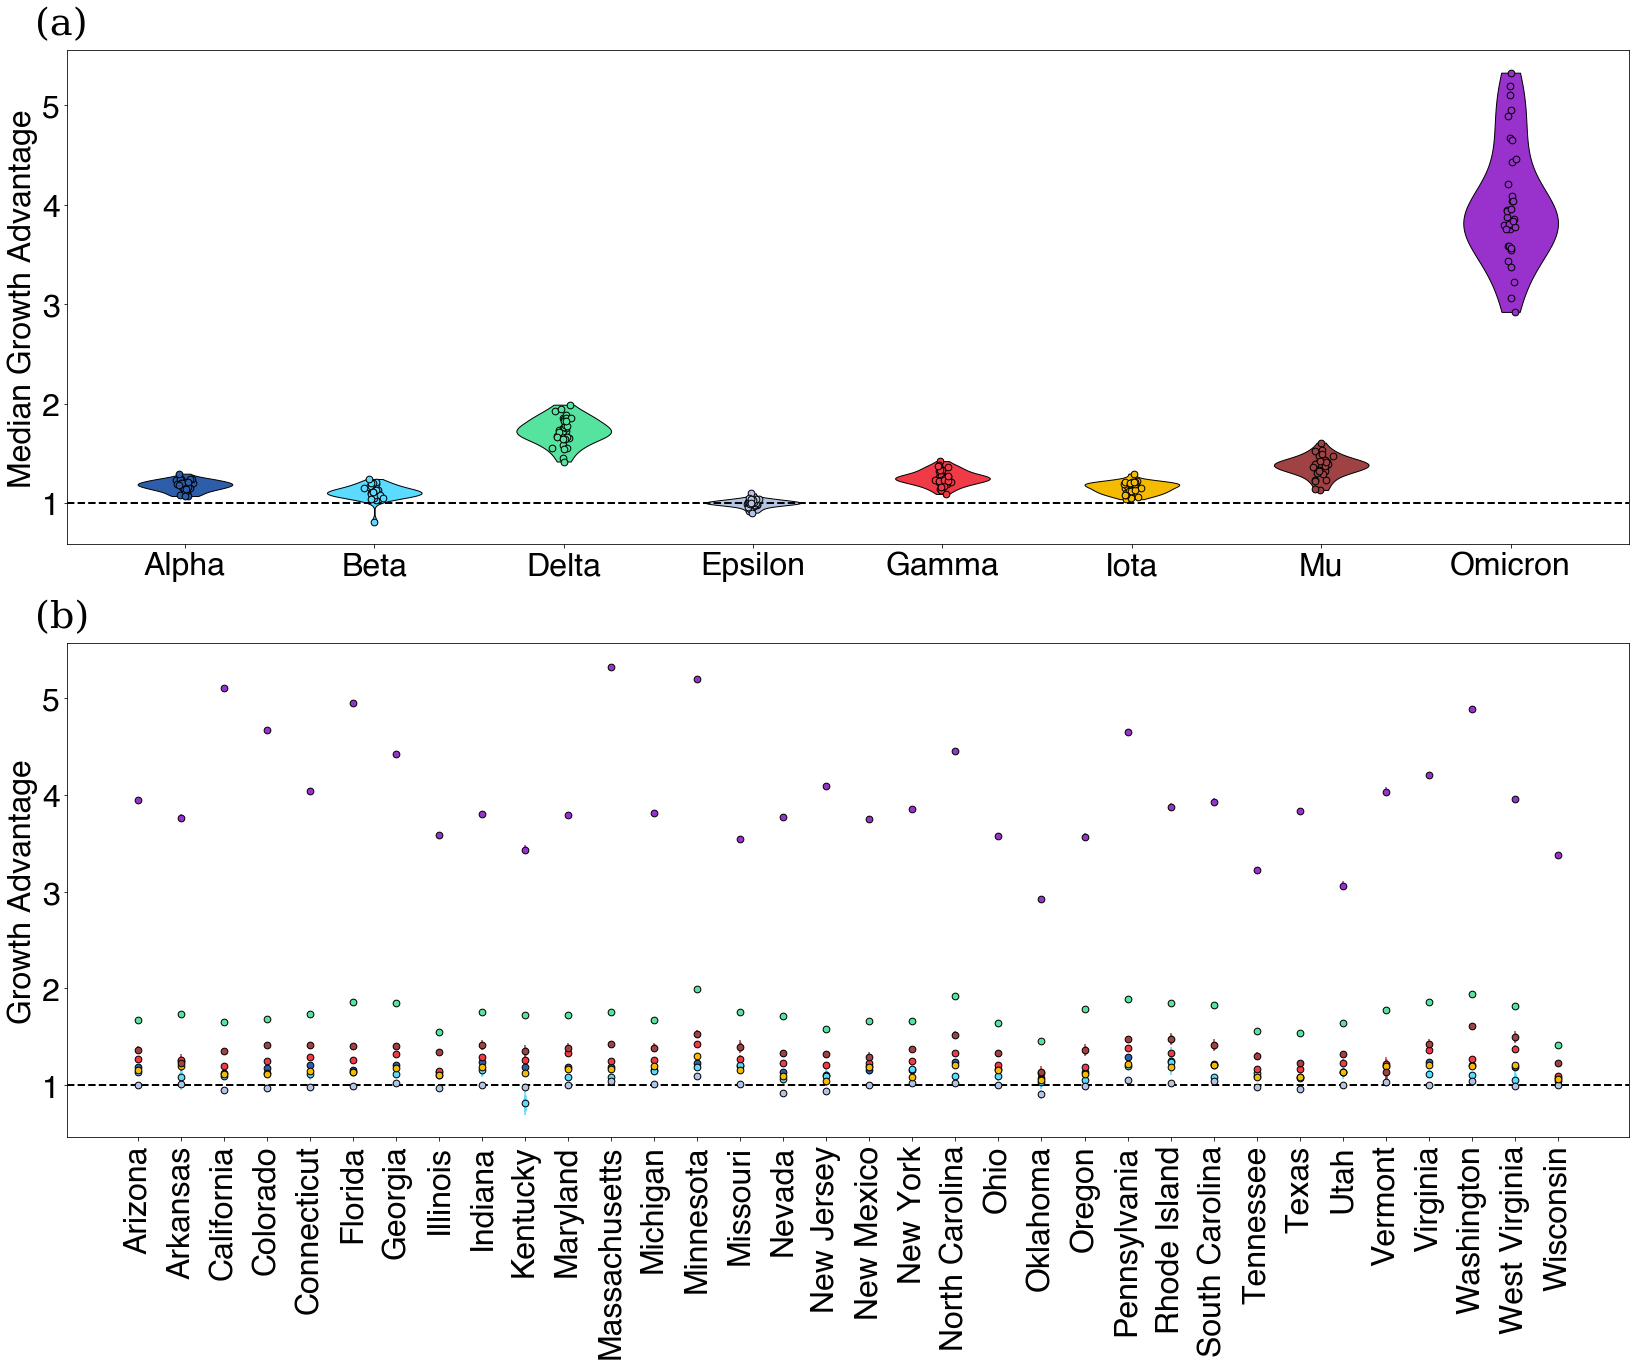
\includegraphics[width=\linewidth]{figs/fig_MLR_growth_advantages_supp.png}
  \caption{\textbf{Estimating variant growth advantages in various states using Multinomial Logistic Regression}
  (a) Growth advantages visualized by state assuming generation time $T_{g} = 5.2$..
  (b) Same as (a) but grouped by variant.}%
  \label{fig:MLR_growth_advantages}
\end{figure}

\newpage

\subsection*{Relating epidemic growth rates to relative effective reproduction numbers}

An important relationship of interest is between the epidemic growth rate of an epidemic and its effective reproduction number.
In the case of our analysis, we are particularly interested in the effect of generation time assumptions on estimated variant-specific effective reproduction numbers.
First, notice that the effective reproduction number and the epidemic growth rate of an epidemic are related by
\begin{align*}
R_{t} = \frac{1}{\int_{0}^{\infty} \exp(-r\tau)g(\tau)d\tau} = \frac{1}{M_{g}(-r)}
\end{align*}
according to the Lotka-Euler equation \cite{Wallinga2006} where $r$ is the epidemic growth rate and $M_{g}$ is the moment-generating function of the generation time $g$.

This allows us to write the relative reproduction number of two variants $v$ and $u$ as a function of their epidemic growth rates, so that
\begin{align*}
\frac{R_{t,v}}{R_{t,u}} = \frac{M_{g}(-r_{u})}{M_{g}(-r_{v})}.
\end{align*}

We'll consider three common generation time assumptions. First, we consider the case where the generation time is a point mass at $T_{g}$. In which case, $M_{g}(-r) = \exp(-r T_{g})$ and we recover the relationship
\begin{align*}
R_{t,v} = \exp(r_{v}T_{g}).
\end{align*}

In this case, the relative effective reproduction number will depend on only the difference between the epidemic growth rates and therefore, is commonly used when converting estimated growth advantages to relative reproduction numbers in the case of logistic growth models.

Second, we consider the case where the generation time is an exponential distribution with mean $T_{g}$. This assumption is often implicit and common in models of infectious diseases such as ODEs and their stochastic variants. Using the corresponding moment-generating function, we see that
\begin{align*}
R_{t,v} = 1 + r_{v} T_{g}
\end{align*}

Next, we consider the Gamma distributed generation times with mean $T_{g}$ and standard deviation $s$.
This is often used in models of infectious diseases via the chain trick in which multiple compartments are chained together to obtain non-exponential generation times or infectious periods.
Re-parameterizing the Gamma distribution in terms of its mean and standard deviation and using its moment generating function, we have that
\begin{align*}
R_{t,v} = \left(1 + r_{v}  \left(\frac{s^{2}}{T_{g}}\right) \right)^{T_{g}^{2} / s^{2}}.
\end{align*}

From this equation, we can see that increases in the mean of the generation time of $v$ leads to decreasing estimates of $R_{t,v}$ during epidemic decline ($r_{v} < 0$) and increased estimates during epidemic growth ($r_{v} > 0$) assuming $r_{v}$ and $s$ are fixed.
Additionally, increases in the standard deviation will generally lead to lower inferred variant advantages.
This effect is also visualized in Figure \ref{fig:generation_time_sensitivity}.

\paragraph{Variant growth-advantages are sensitive to generation time}%

In the case where we have two variants $u, v$ with Gamma-distributed generation times with means $T_{u}, T_{v}$ and standard deviations $s_{u}, s_{v}$ respectively, we can then write the relative effective reproduction number of $v$ over $u$ as
\begin{align*}
\frac{R_{t,v}}{R_{t,u}} = \frac{\left[1 + r_{v}  \left(\frac{s_{v}^{2}}{T_{v}}\right)\right]^{T_{v}^{2} / s_{v}^{2}}}{\left[1 + r_{u} \left(\frac{s_{u}^{2}}{T_{u}}\right)\right]^{T_{u}^{2} / s_{u}^{2}}}.
\end{align*}
It follows that increases in the mean of the generation time of $v$ leads to decreasing inferred variant advantages during epidemic decline and increased advantages during epidemic growth when all quantities are fixed.
On the other hand, increases in the standard deviation will generally lead to lower inferred variant advantages.

Taking a logarithm, we can also evaluate the sensitivity of our inferred growth advantages from our fixed growth advantage model with respect to the generation time assuming it is Gamma distributed as
\begin{align*}
 \delta_{v}  = \ln \left( \frac{R_{t,v}}{R_{t,0}} \right) = \left( \frac{T_{g}^{2}}{s^{2}} \right)  \ln \left( \frac{1 + r_{v}  \left(\frac{s^{2}}{T_{g}}\right)}{1 + r_{0} \left(\frac{s^{2}}{T_{g}}\right) } \right).
\end{align*}
As the log of the relative effective reproduction number, the behavior here is analogous to that discussed above when the mean $T_{g}$ and standard deviation $s$ are changed.
This effects of varying mean and standard deviation are illustrated in Figure \ref{fig:growth_advantage_sensitivity}.
Although the effective reproduction number and the growth advantage appear to have strong dependence on generation time parameters, we find that the epidemic growth rate $r$ is more robust to changes in generation time (see Figure \ref{fig:little_r_sensitivity}).

The cases of exponential and Gamma-distributed generation times highlight that for non-deterministic generation times there is no guarantee that the relative effective reproduction number depends on only the difference in epidemic growth rates.
In fact, these estimates based on the deterministic generation times correspond to the case in which the standard deviation shrinks zero, they are likely overestimates of variant advantages given the observed variation in the serial interval of SARS-CoV-2 infections.

\paragraph{Fixed growth advantages become time-varying under generation time misspecification}

We'll now consider the case where there is a true fixed-variant growth advantage. Suppose for a two-variant system that $\delta$ is the constant (log) growth advantage of the variant virus over the wildtype under the variant generation time $g_{T}$, so that $\delta = \ln \left( R_{t,v}^{g_{T}} / R_{t, wt}^{g_{T}} \right)$.
Here subscripts denote the generation time used when computing $R_{t}$.

Under the misspecified variant generation time $g_{M}$, we can then write the inferred growth advantage as
\begin{align*}
  \delta_{M} &= \ln \left( \frac{R_{t,v}^{g_{M}}}{R_{t, wt}^{g_{T}}} \right) = \ln \left(\frac{R_{t,v}^{g_{M}}}{R_{t,v}^{g_{T}}}\right) + \delta.
\end{align*}

In general, the term inside the log is non-constant meaning that fixed variant growth advantages under one generation time become non-constant under generation time specification.

\begin{figure}
  \centering
  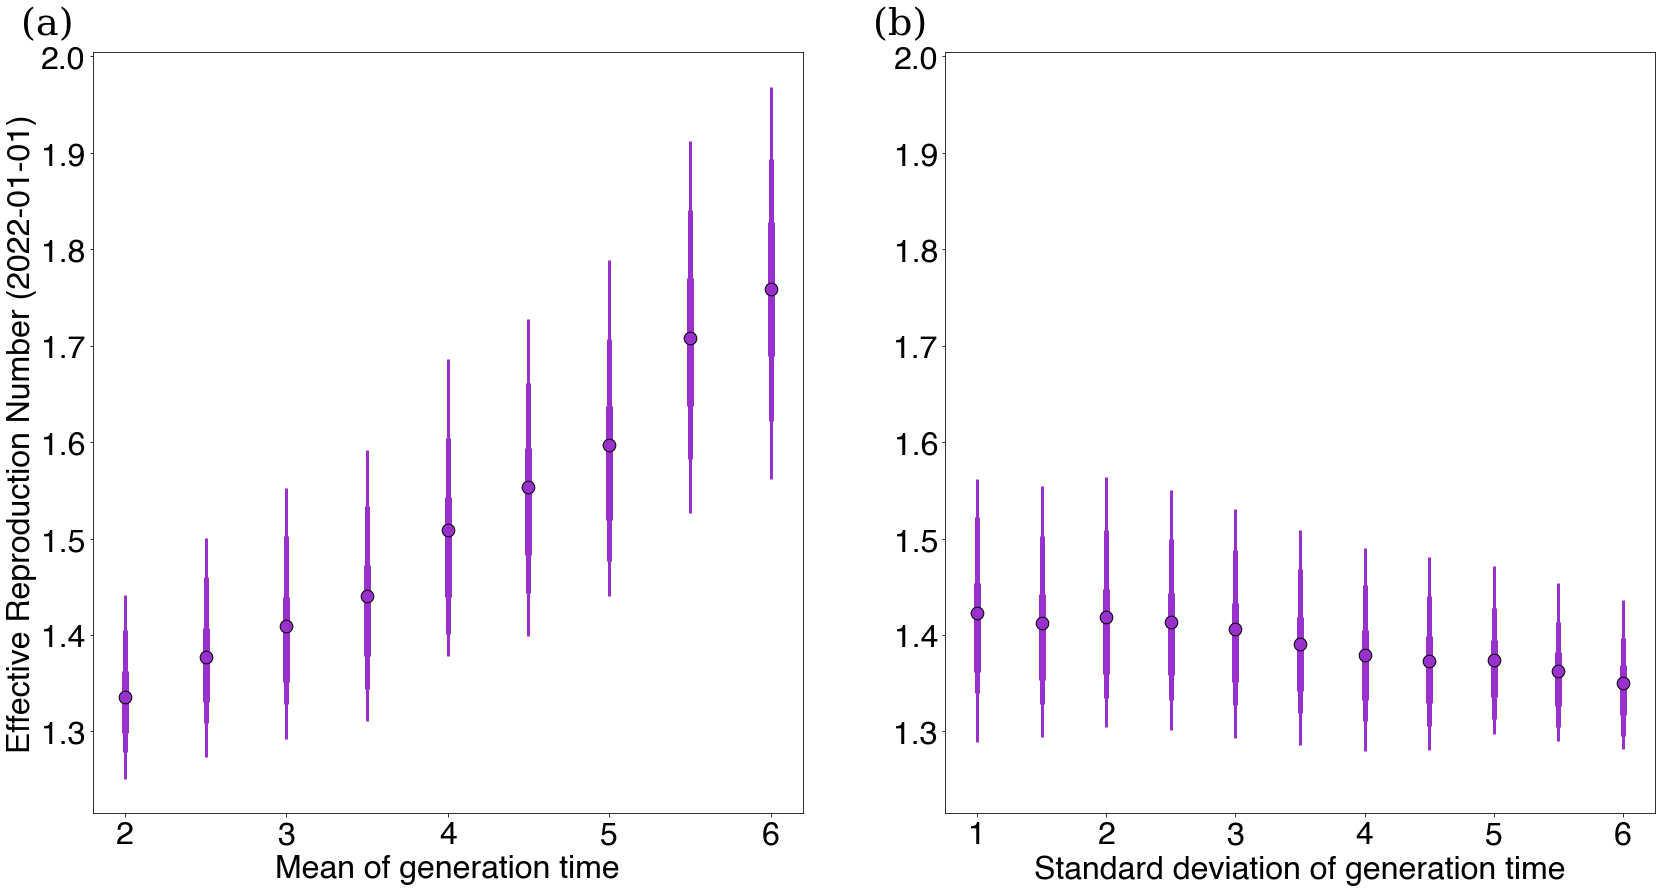
\includegraphics[width=\linewidth]{figs/generation_time_sensitivity.png}
  \caption{\textbf{Sensitivity of effective reproduction number to changes in generation time.}
(a) We vary the mean of Omicron generation time keeping a constant standard deviation 1.2 and plot against effective reproduction number estimates for Omicron in Washington state on February 1st, 2022 using our GARW model.
(b) The same as (a), but we instead vary the standard deviation of Omicron generation time keeping a constant mean 3.1.}%
  \label{fig:generation_time_sensitivity}
\end{figure}

\begin{figure}
  \centering
  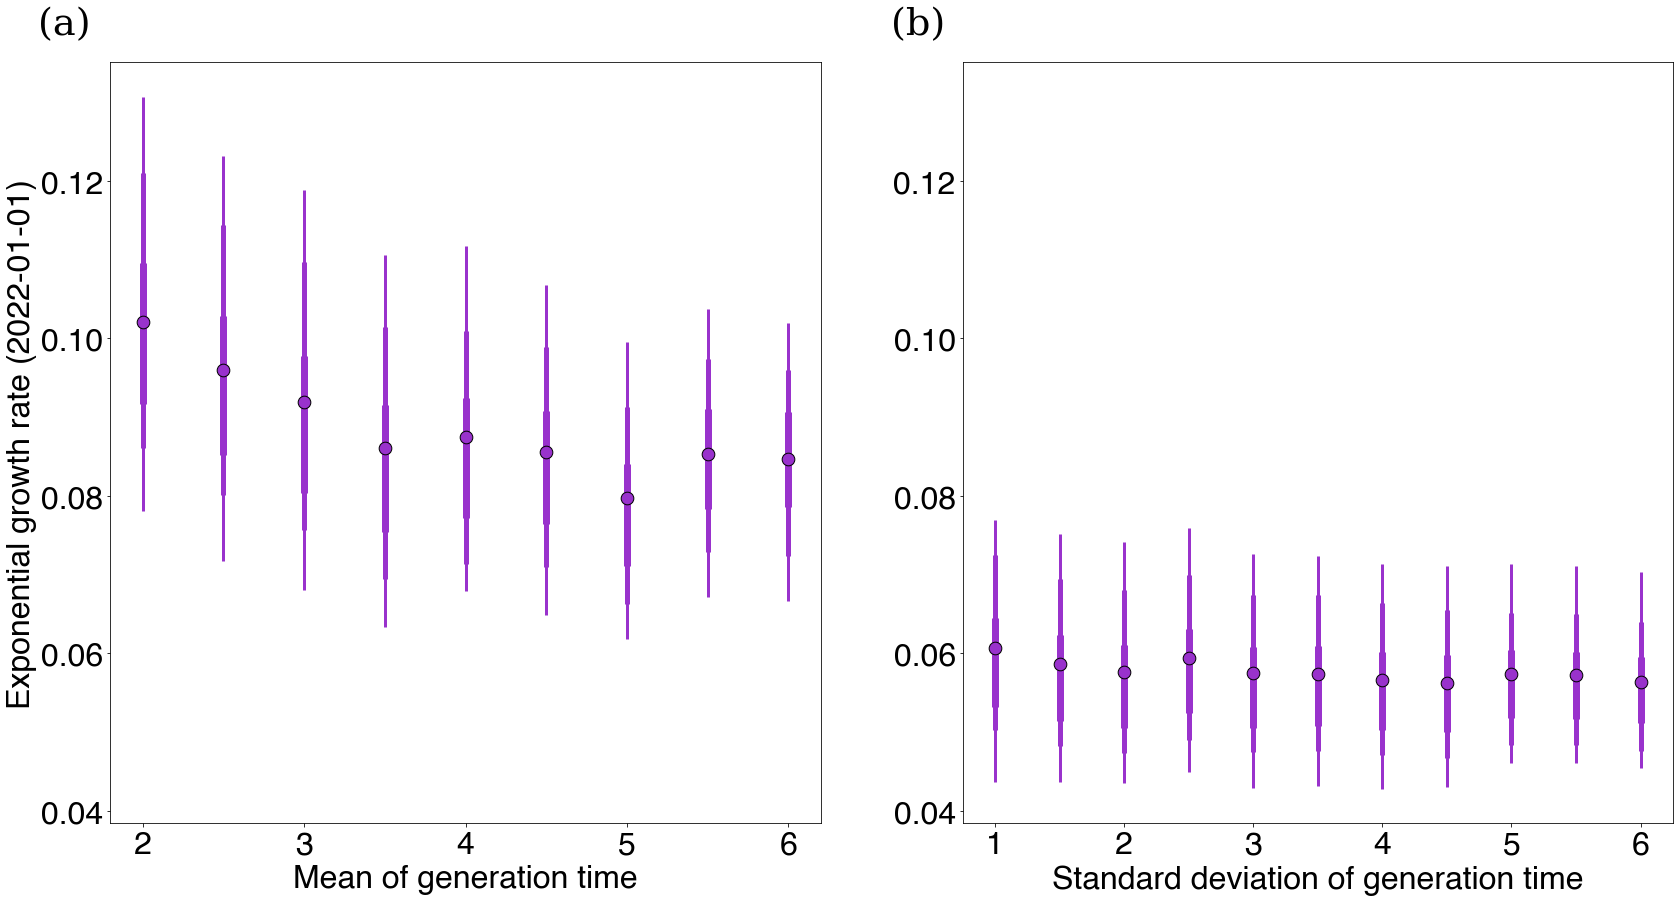
\includegraphics[width=\linewidth]{figs/little_r_sensitivity.png}
  \caption{\textbf{Sensitivity of epidemic growth rates to changes in generation time.}
(a) We vary the mean of Omicron generation time keeping a constant standard deviation 1.2 and plot against exponential growth rates for Omicron in Washington state on February 1st, 2022 using our GARW model and assuming a Gamma-distributed generation time.
(b) The same as (a), but we instead vary the standard deviation of Omicron generation time keeping a constant mean 3.1. }%
  \label{fig:little_r_sensitivity}
\end{figure}

\begin{figure}
  \centering
  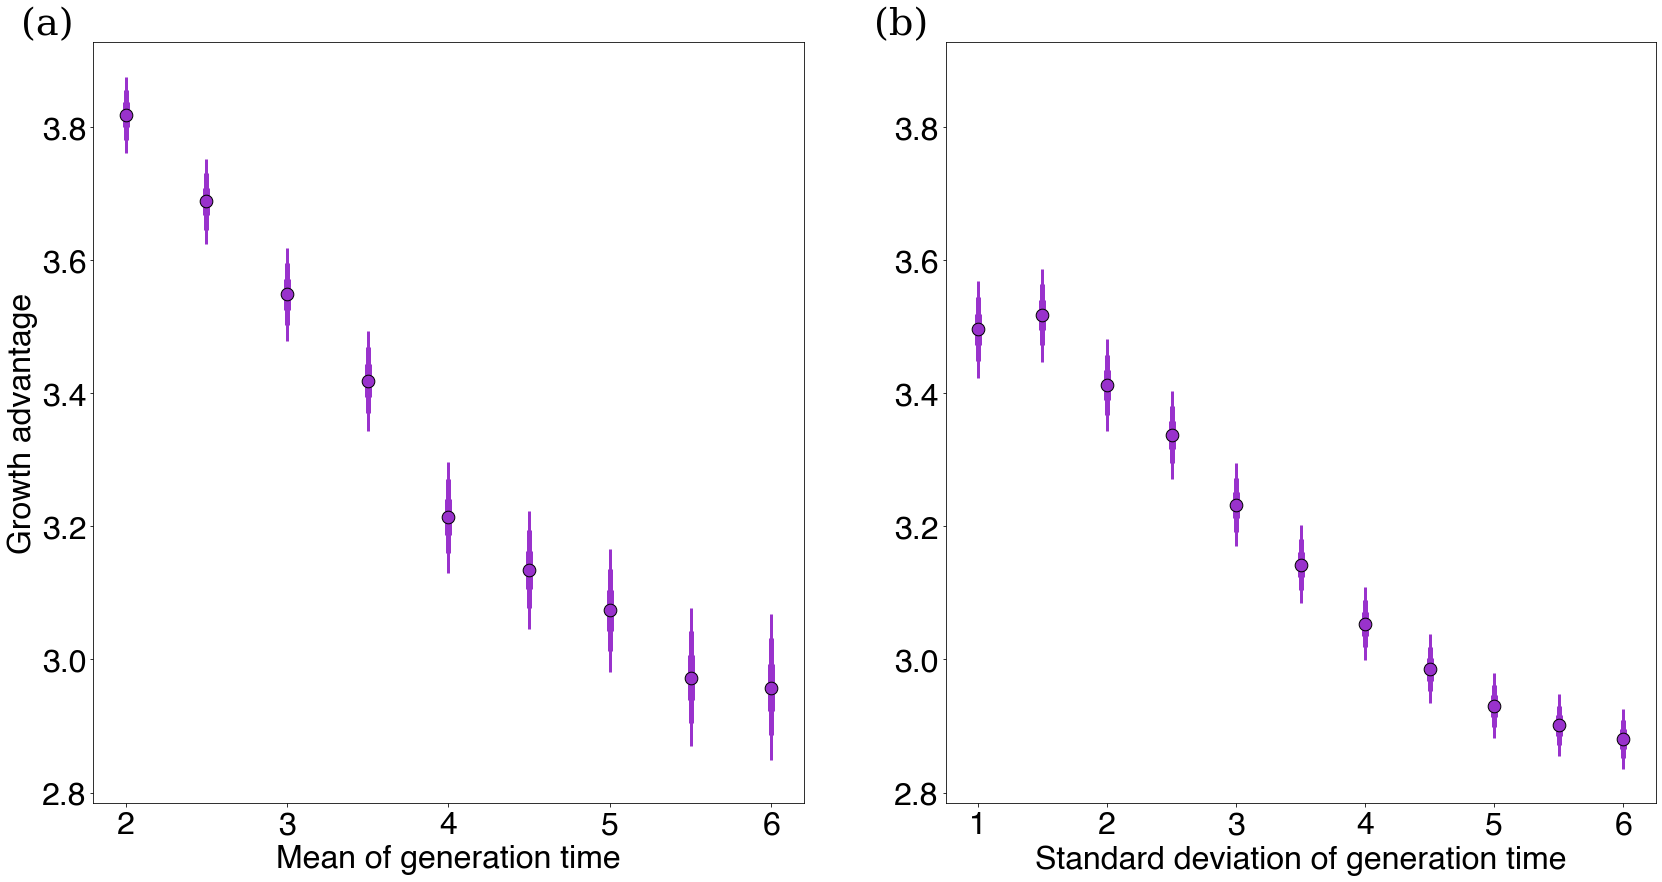
\includegraphics[width=\linewidth]{figs/growth_advantage_sensitivity.png}
  \caption{\textbf{Sensitivity of growth advantages to changes in generation time.}
(a) We vary the mean of Omicron generation time keeping a constant standard deviation 1.2 and plot against exponential growth rates for Delta in Washington state on July 1st, 2021 using our fixed growth model.
(b) The same as (a), but we instead vary the standard deviation of Omicron generation time keeping a constant mean 3.2.}%
  \label{fig:growth_advantage_sensitivity}
\end{figure}

\section{Supplementary Figures}

\begin{figure}
  \centering
  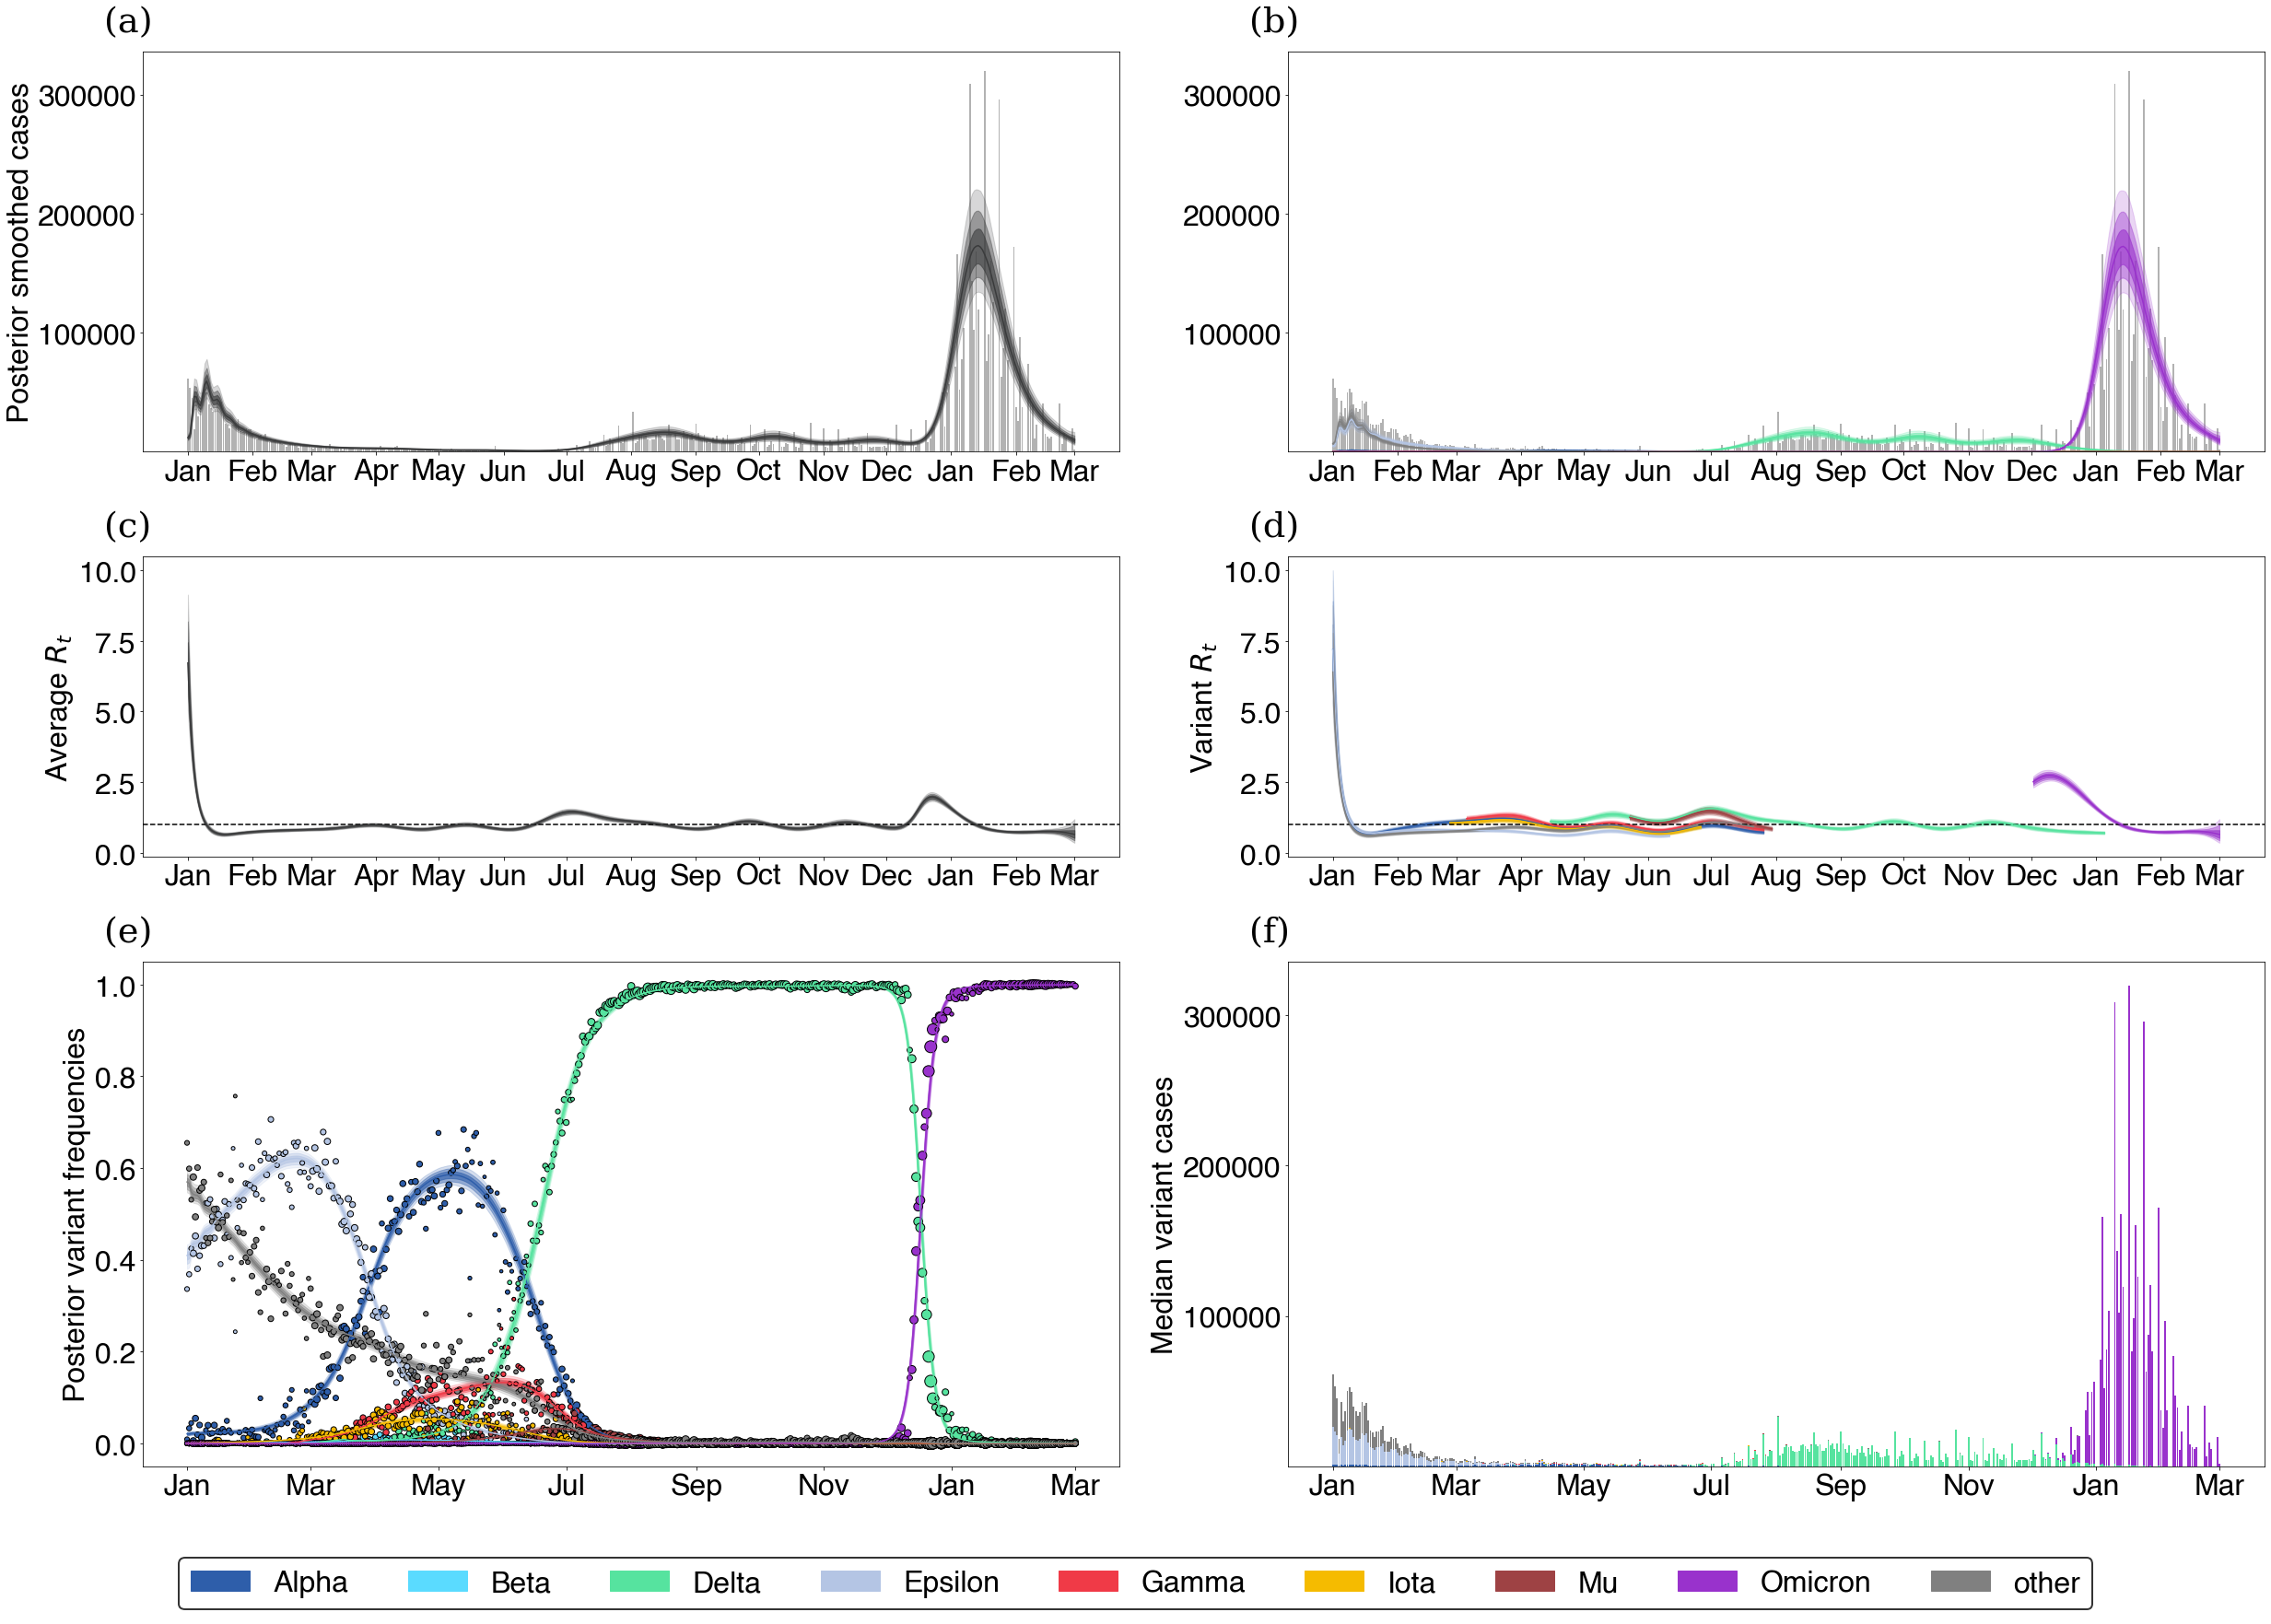
\includegraphics[width=\linewidth]{figs/GARW_rt_California.png}
  \caption{\textbf{Fitting the GARW model to California data.}}%
  \label{fig:GARW_rt_California}
\end{figure}

\begin{figure}
  \centering
  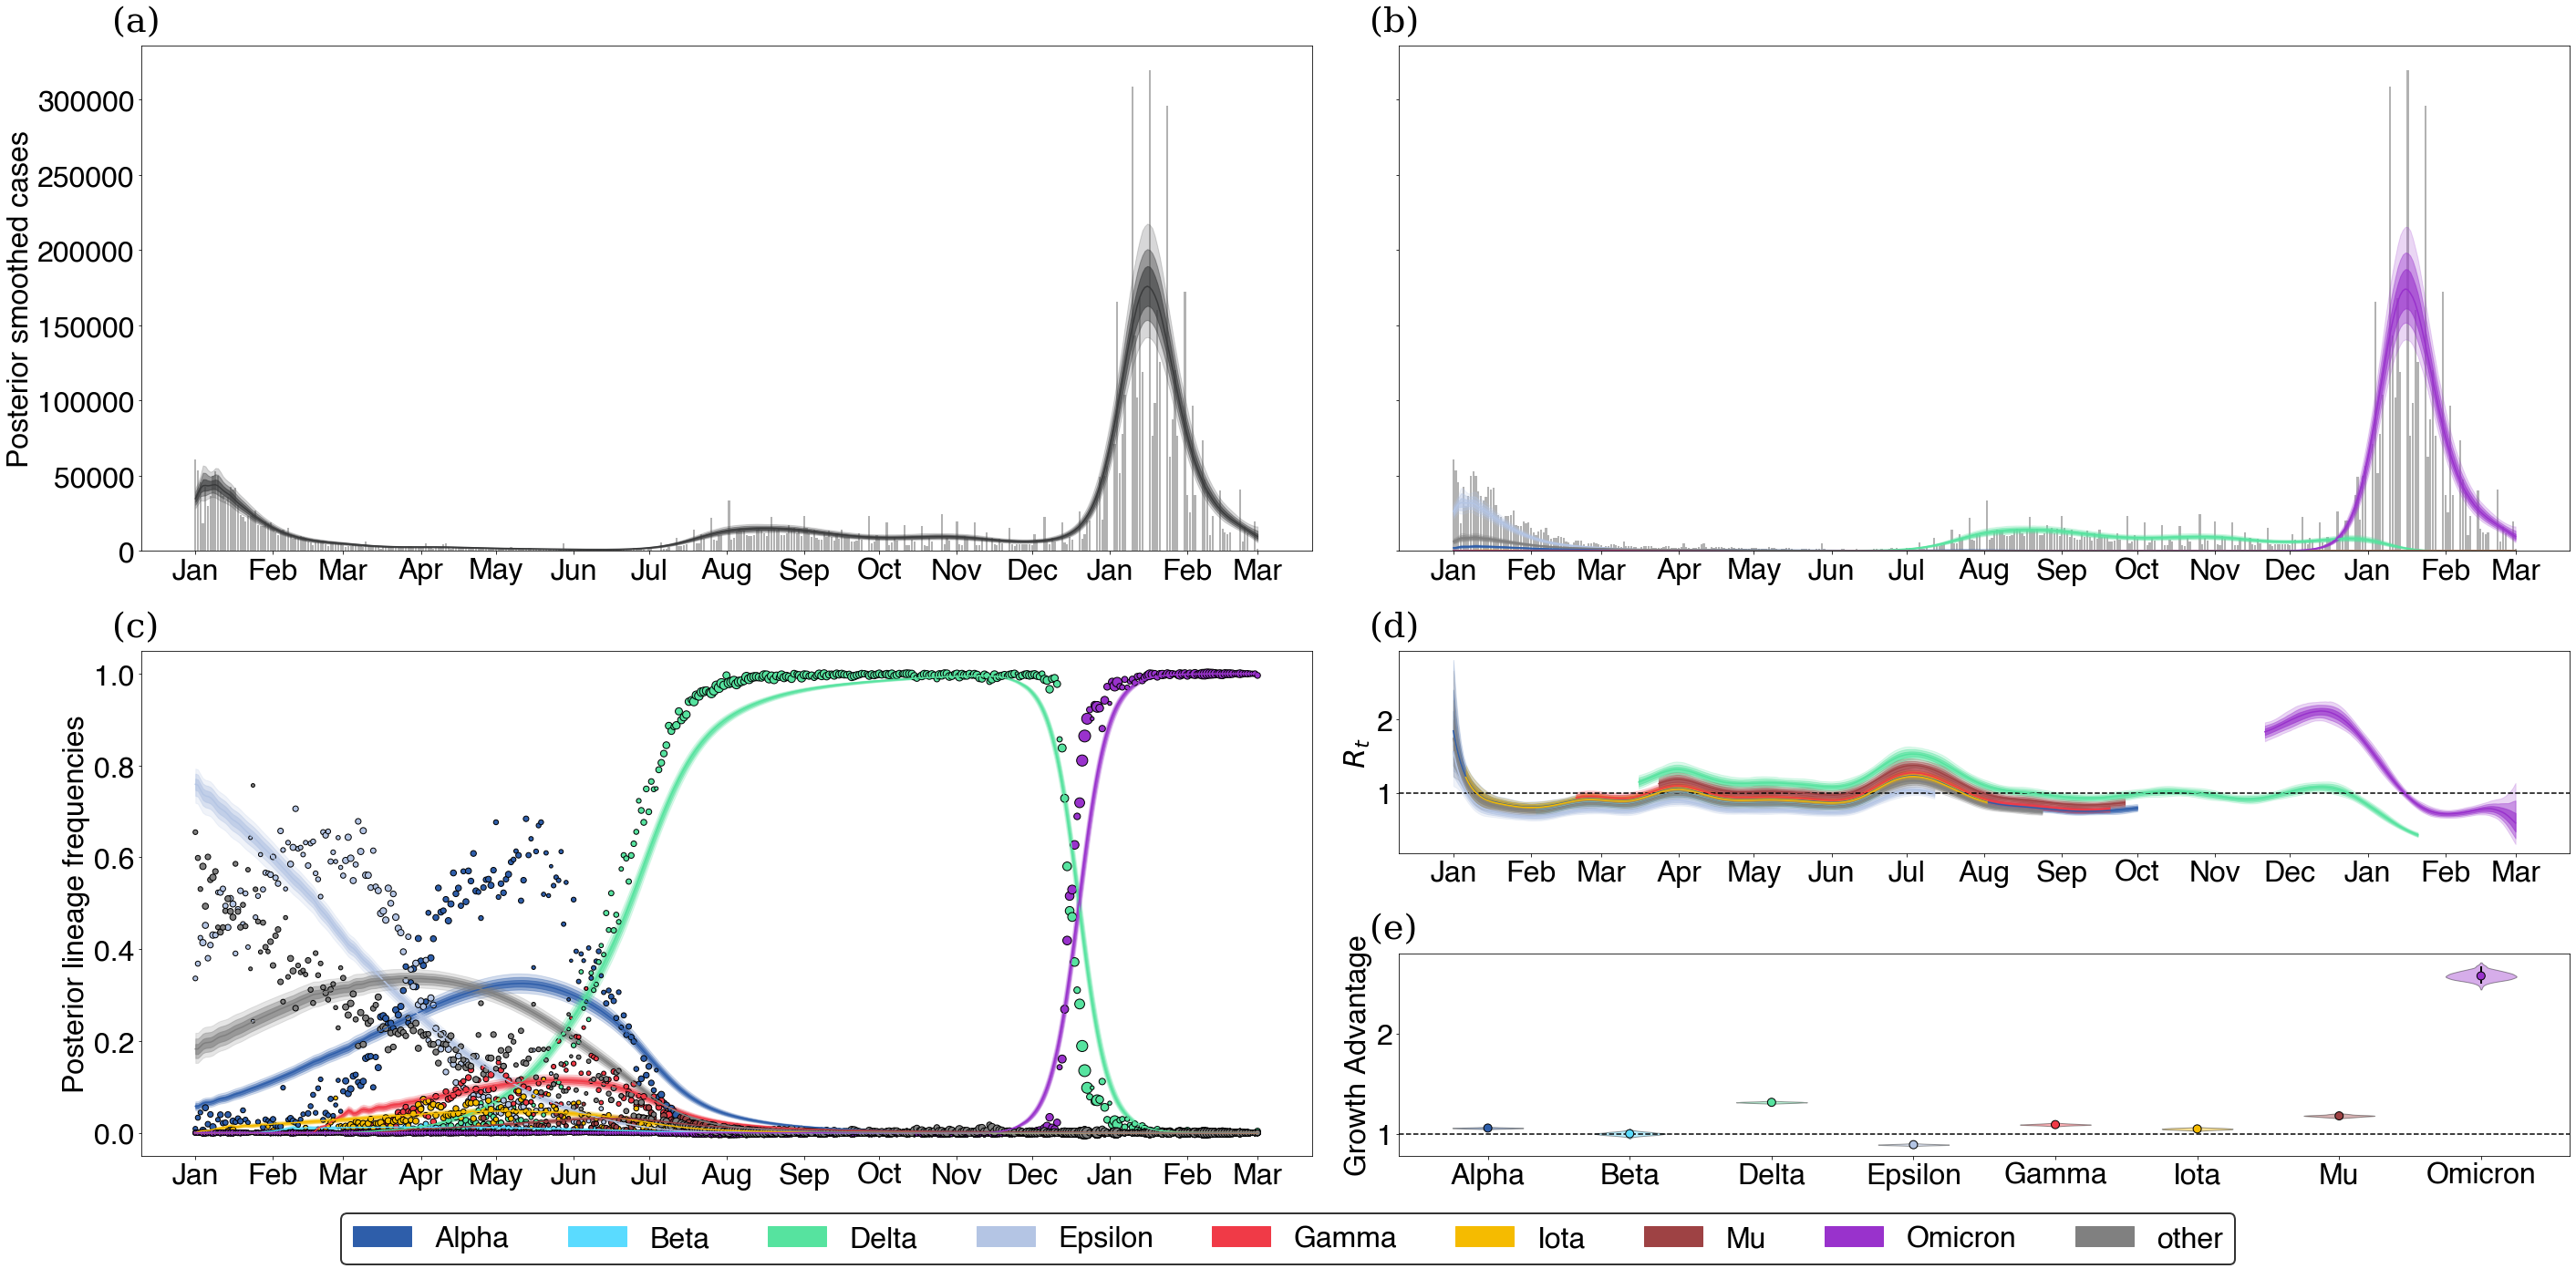
\includegraphics[width=\linewidth]{figs/fixed_growth_California.png}
  \caption{\textbf{Fitting the fixed growth advantage model to California data.}}%
  \label{fig:fixed_growth_California}
\end{figure}

\begin{figure}
  \centering
  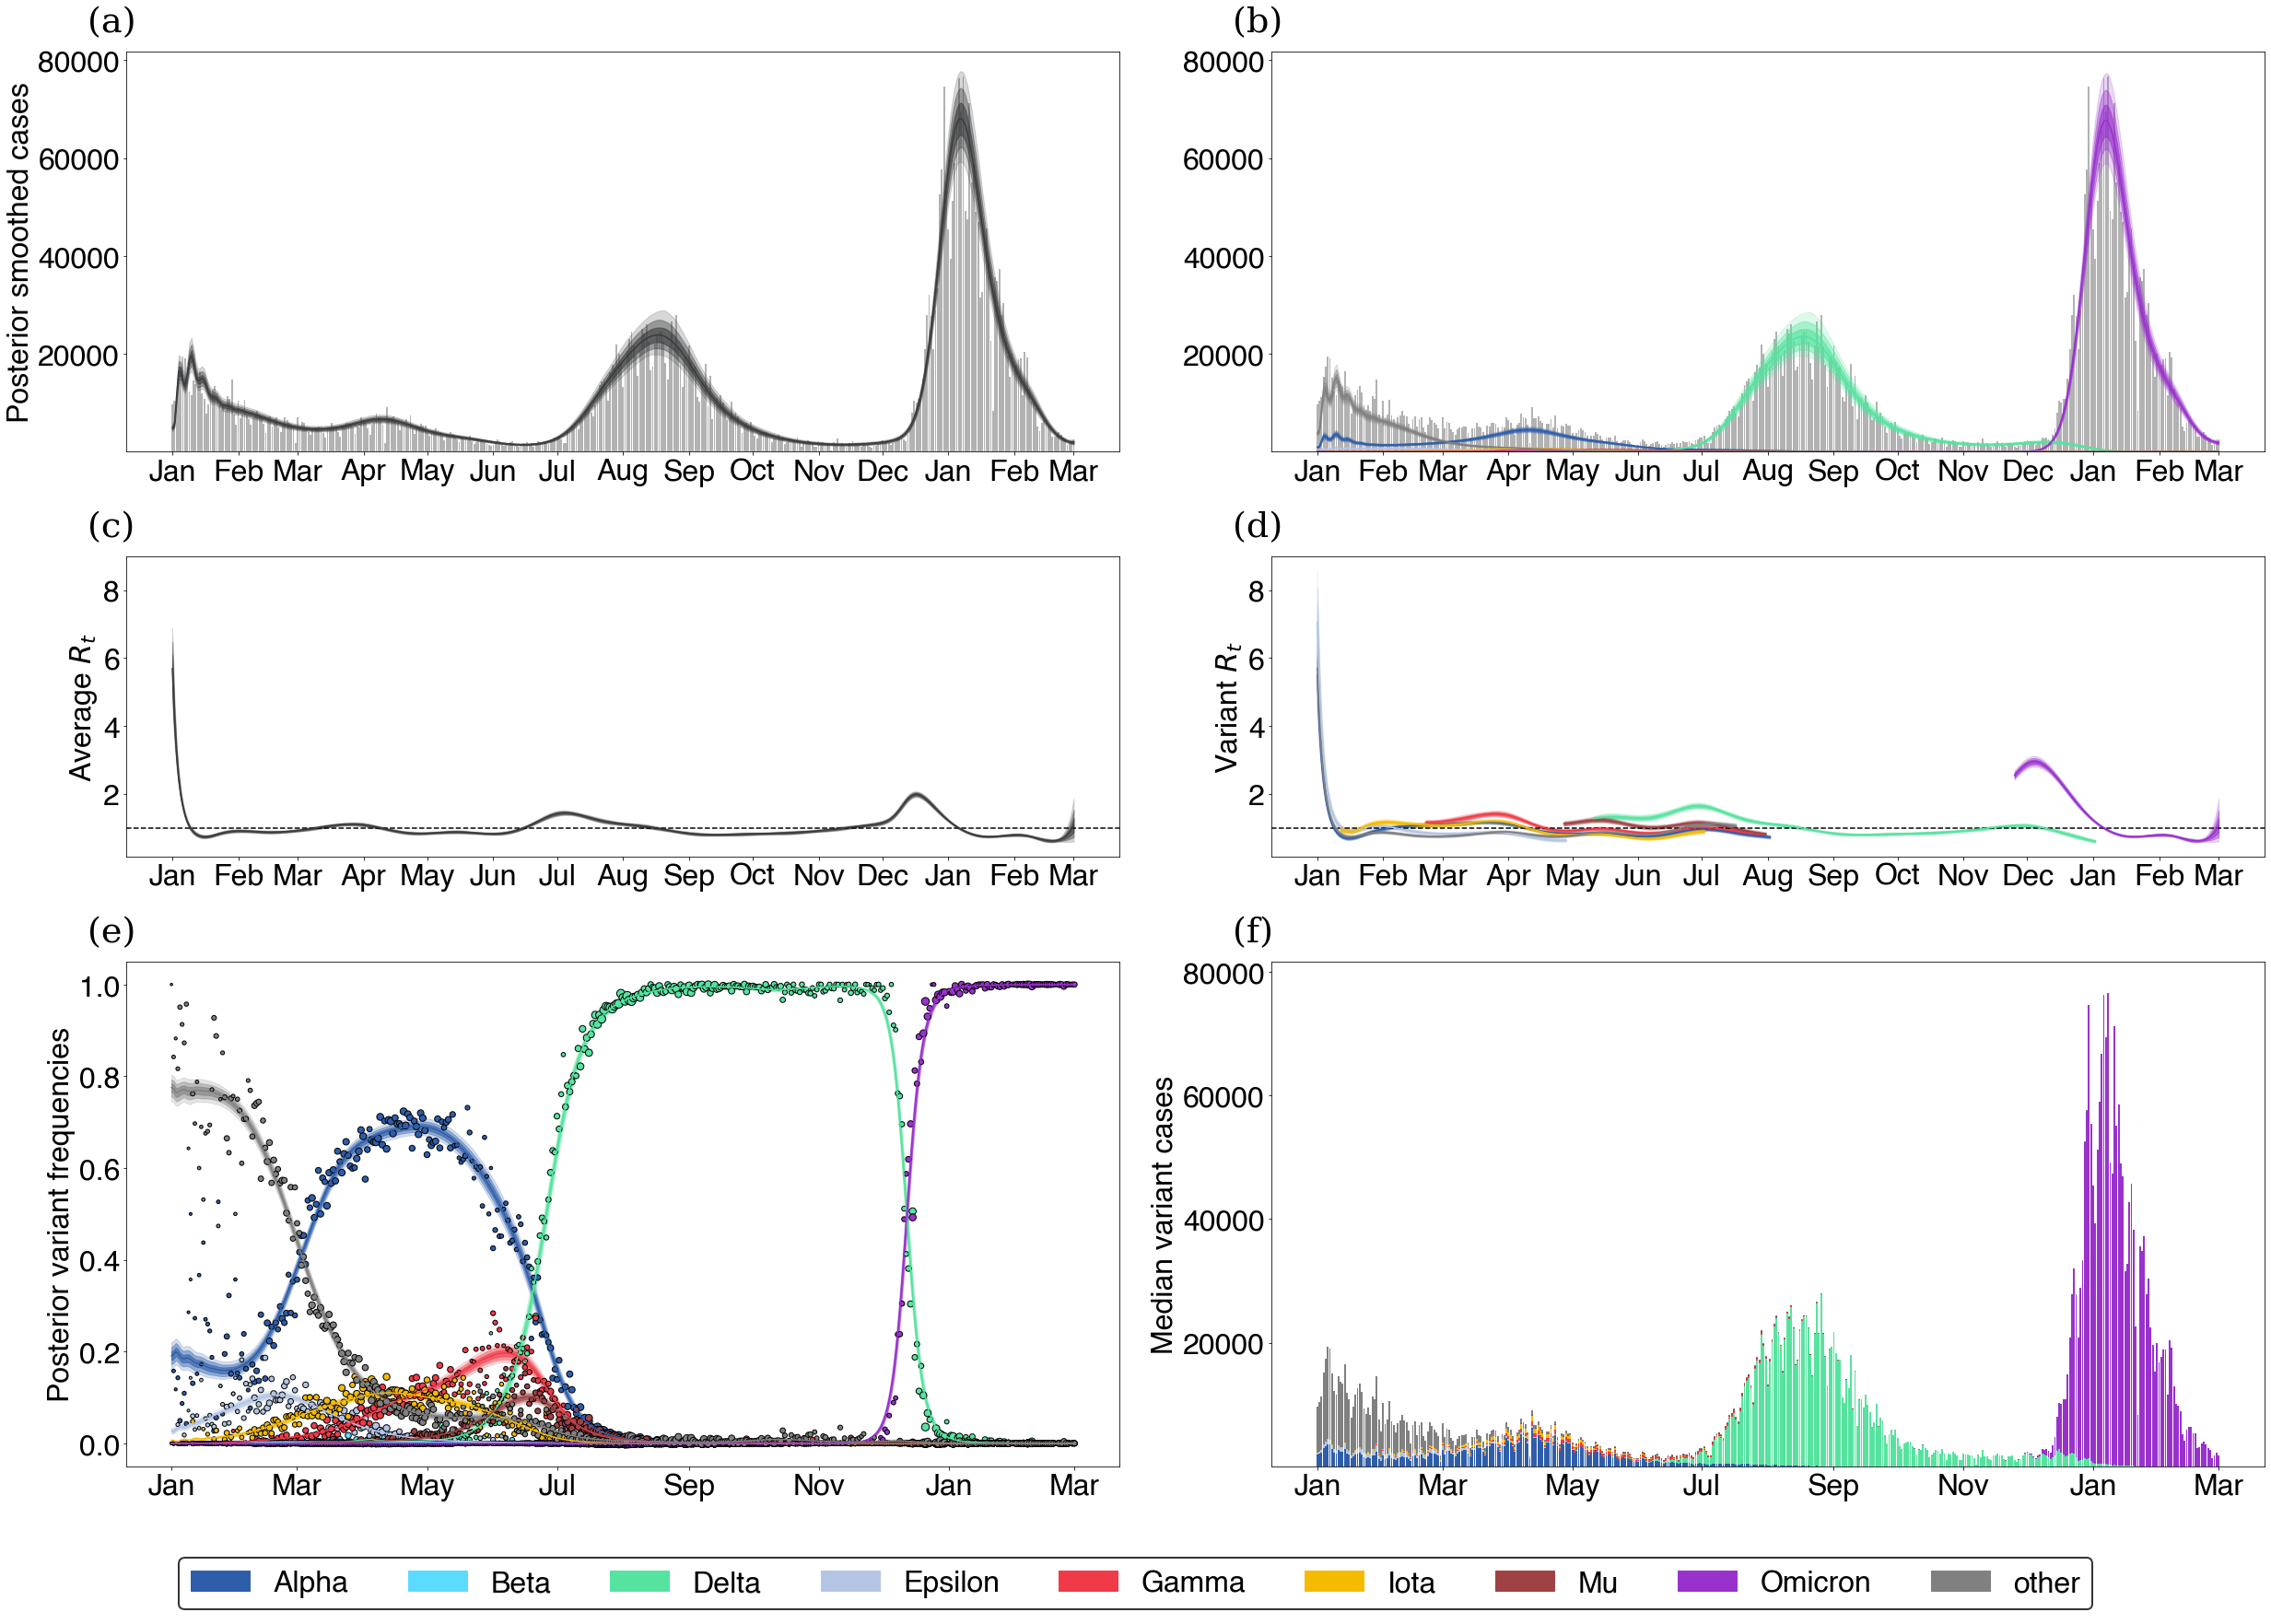
\includegraphics[width=\linewidth]{figs/GARW_rt_Florida.png}
  \caption{\textbf{Fitting the GARW model to Florida data.}}%
  \label{fig:GARW_rt_Florida}
\end{figure}

\begin{figure}
  \centering
  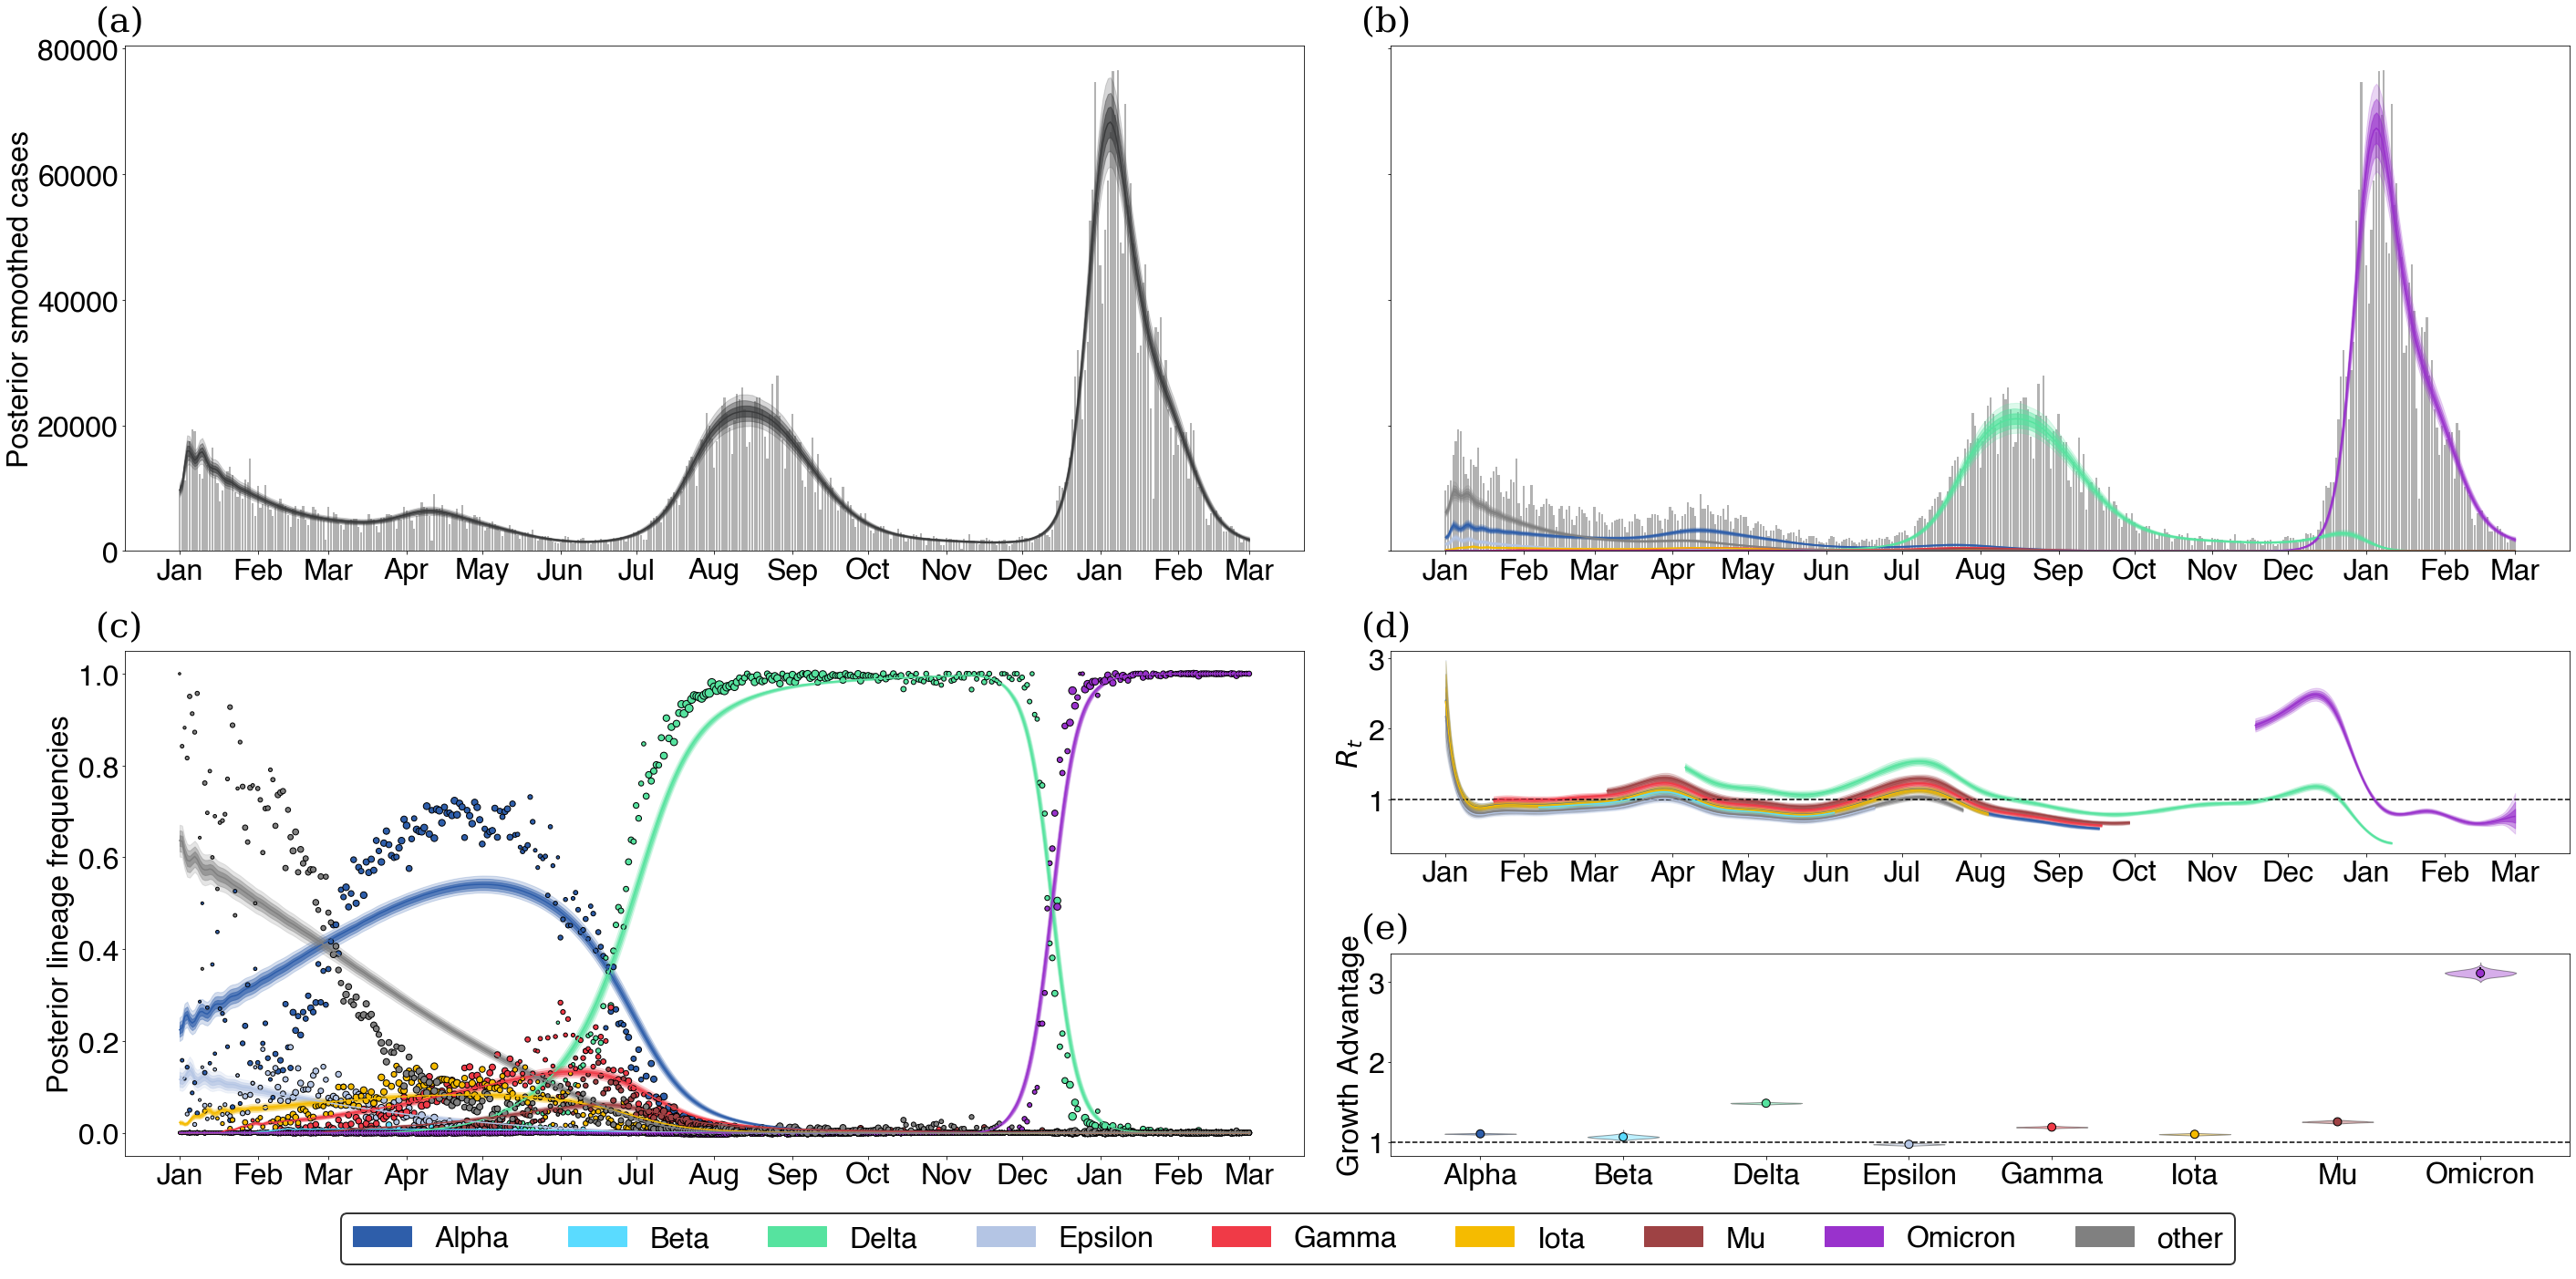
\includegraphics[width=\linewidth]{figs/fixed_growth_Florida.png}
  \caption{\textbf{Fitting the fixed growth advantage model to Florida data.}}%
  \label{fig:fixed_growth_Florida}
\end{figure}

\begin{figure}
  \centering
  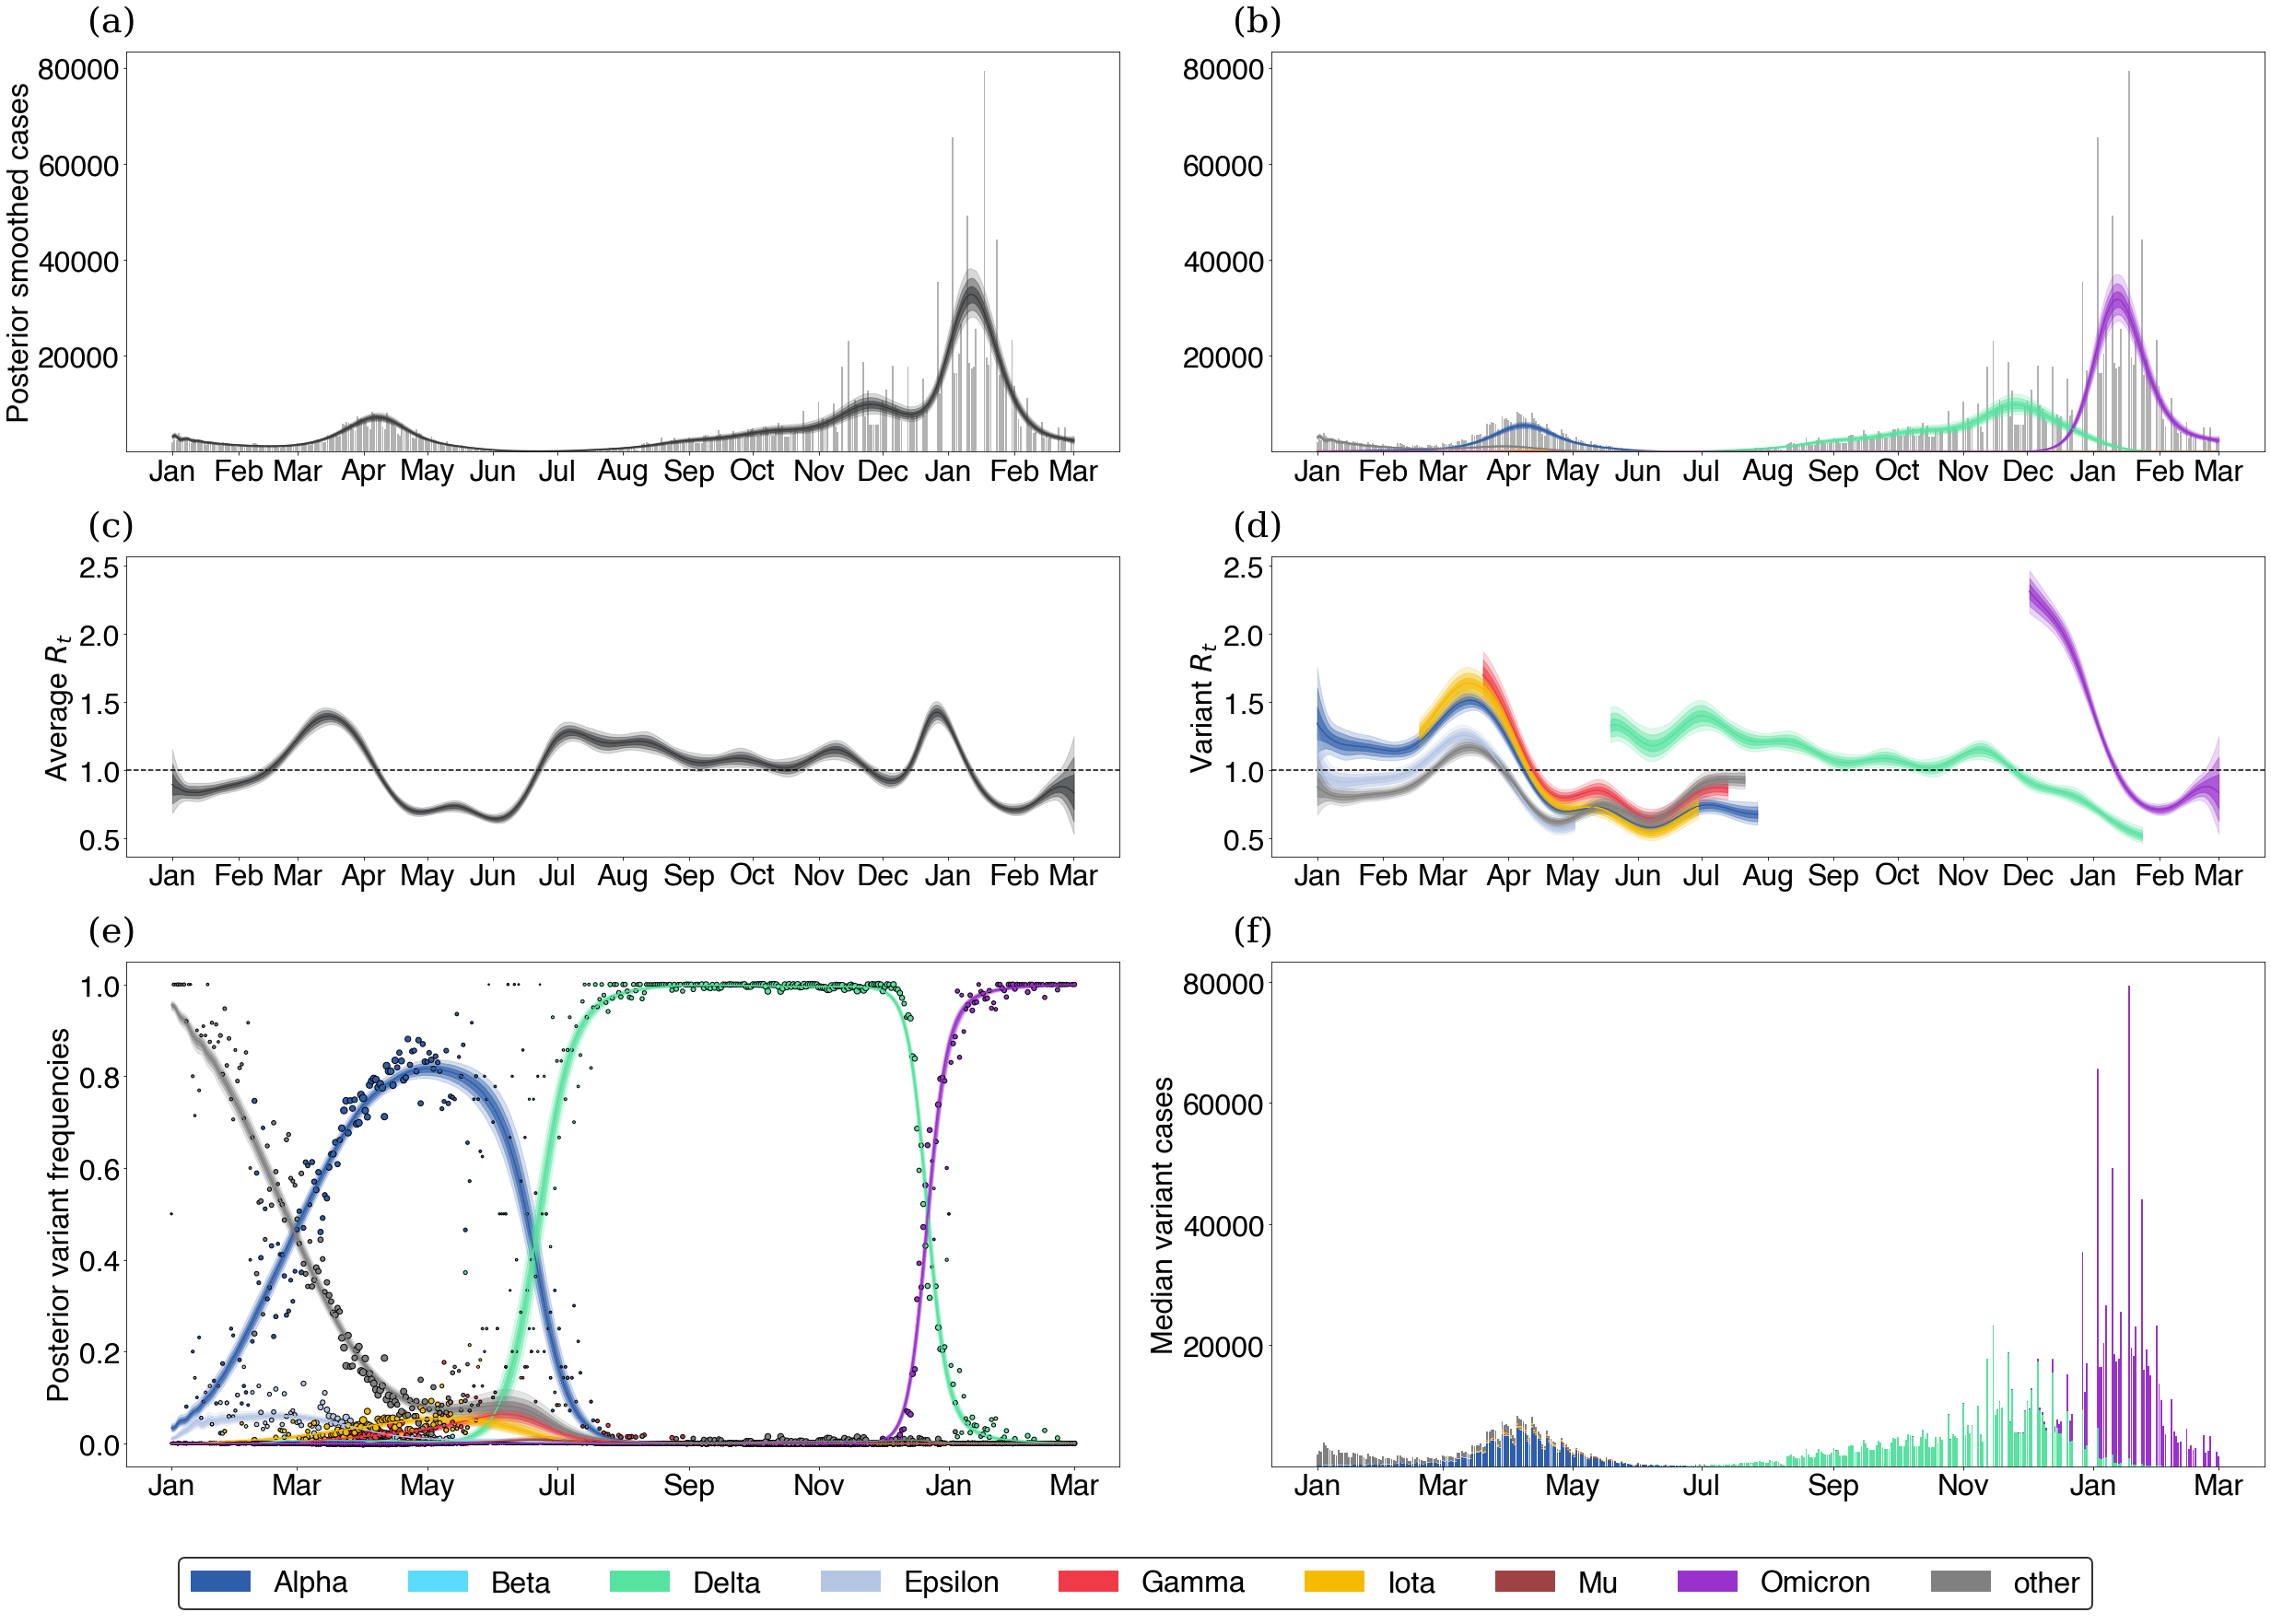
\includegraphics[width=\linewidth]{figs/GARW_rt_Michigan.png}
  \caption{\textbf{Fitting the GARW model to Michigan data.}}%
  \label{fig:GARW_rt_Michigan}
\end{figure}

\begin{figure}
  \centering
  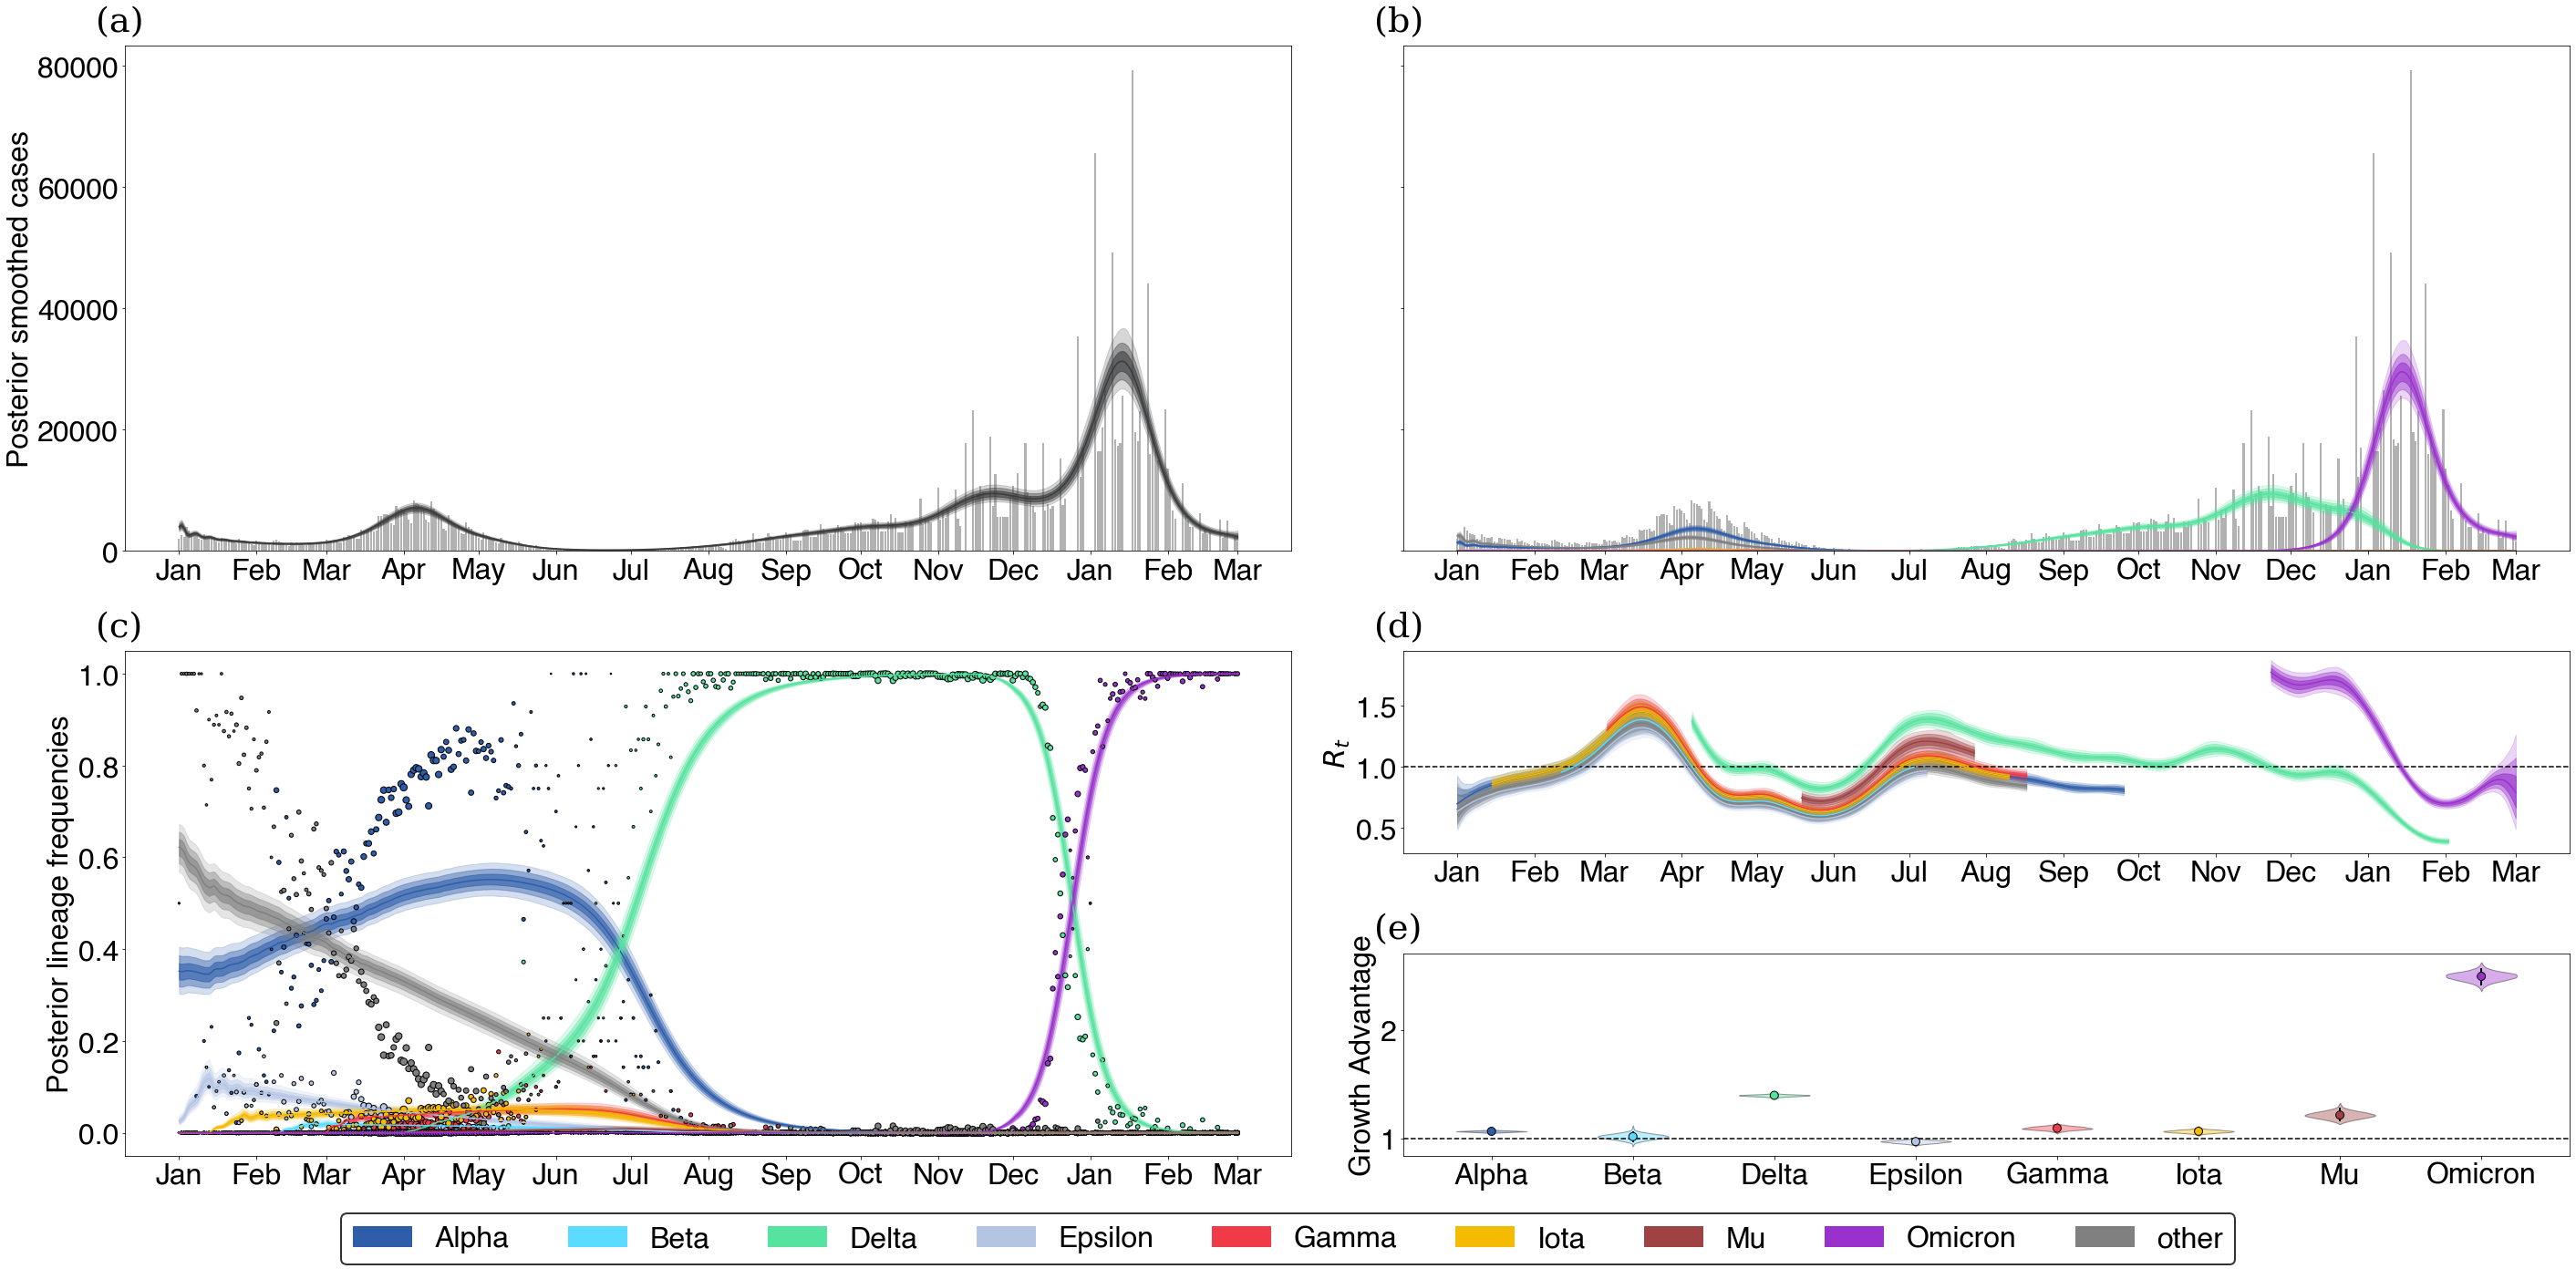
\includegraphics[width=\linewidth]{figs/fixed_growth_Michigan.png}
  \caption{\textbf{Fitting the fixed growth advantage model to Michigan data.}}%
  \label{fig:fixed_growth_Michigan}
\end{figure}

\begin{figure}
  \centering
  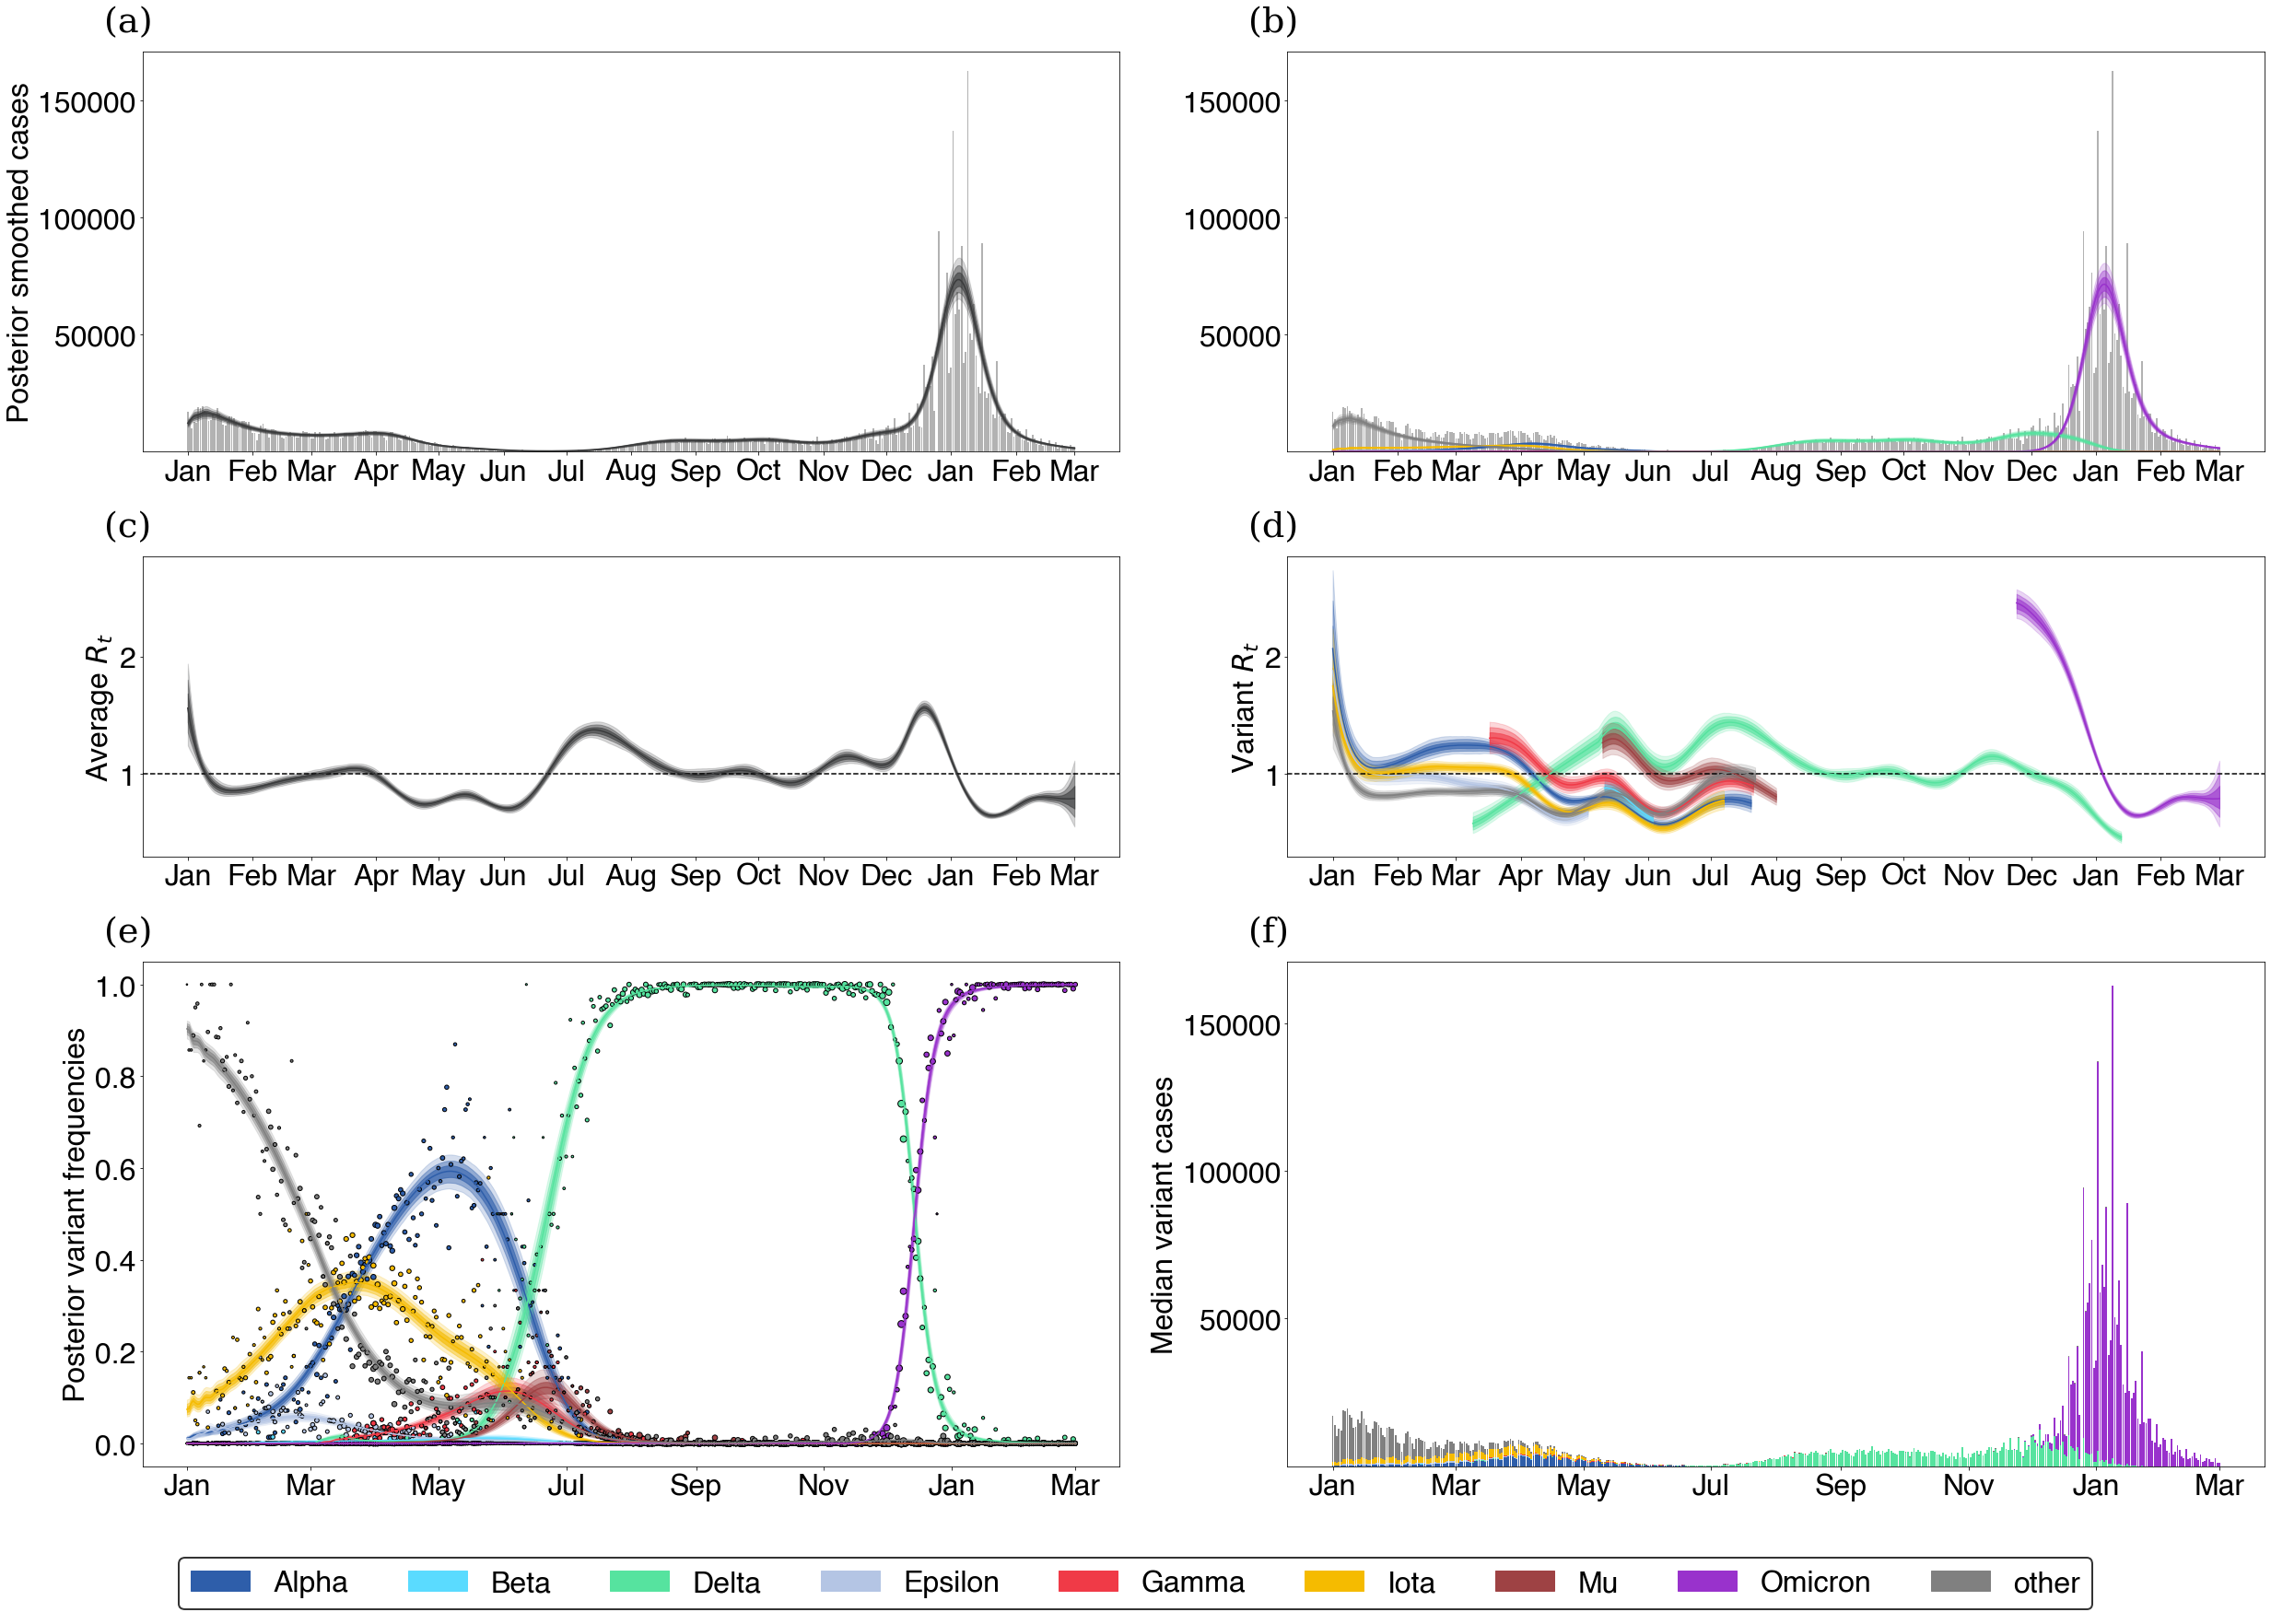
\includegraphics[width=\linewidth]{figs/GARW_rt_New-York.png}
  \caption{\textbf{Fitting the GARW model to New York state data.}}%
  \label{fig:GARW_rt_New-York}
\end{figure}

\begin{figure}
  \centering
  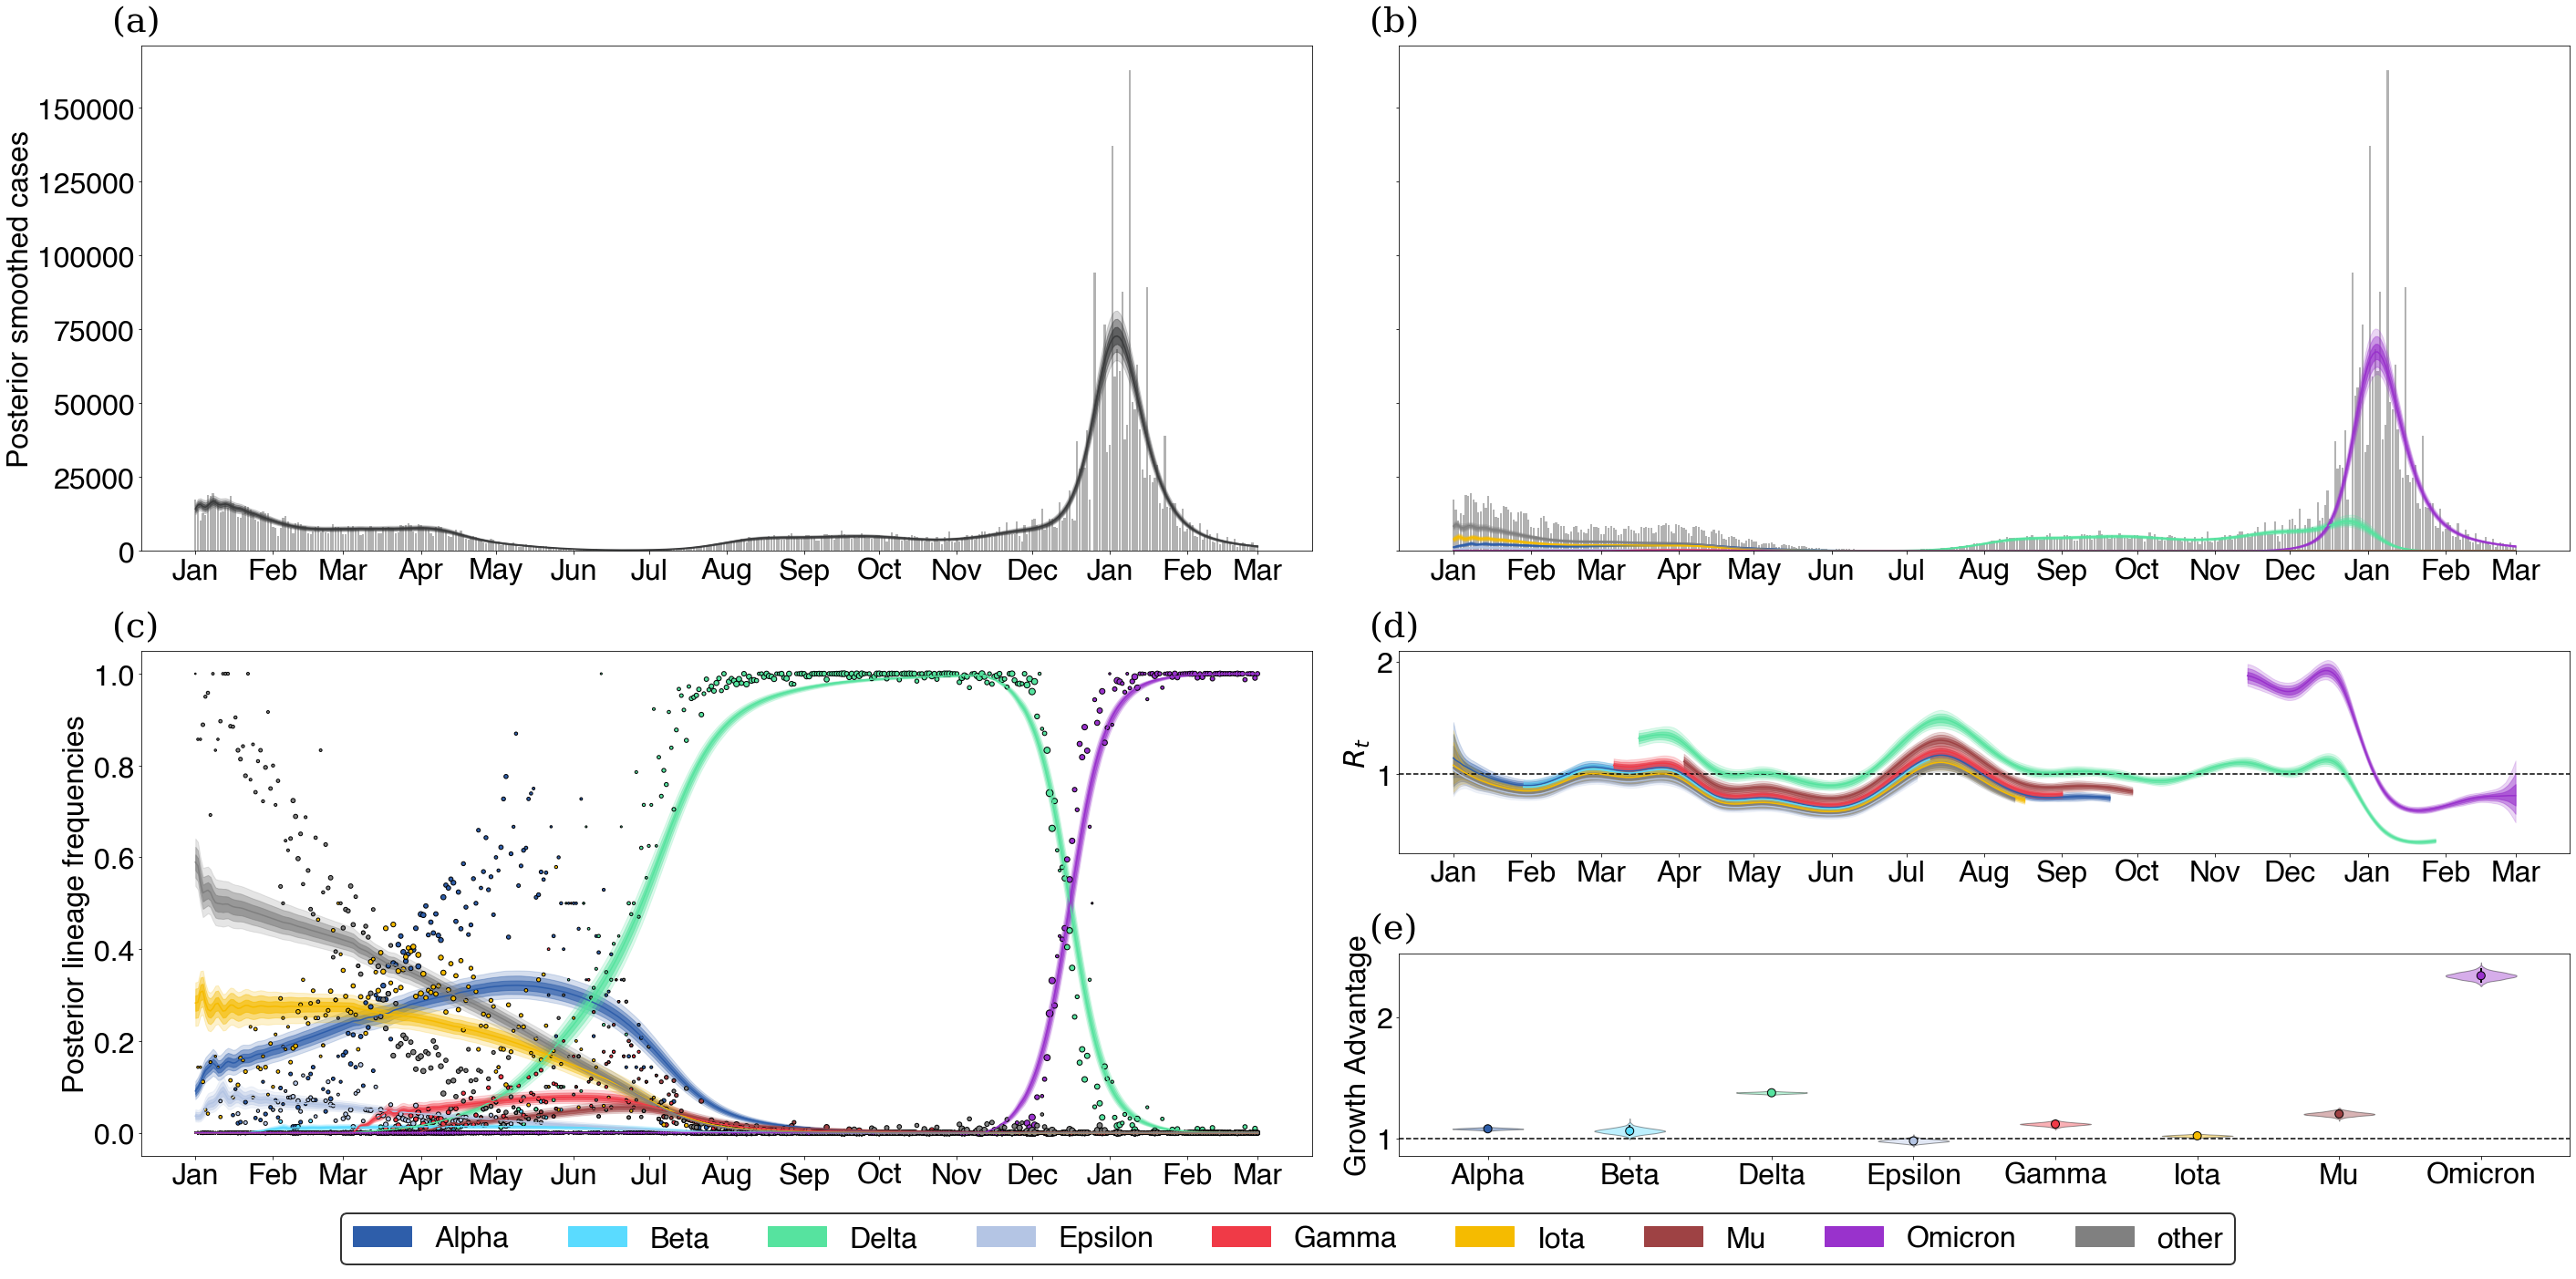
\includegraphics[width=\linewidth]{figs/fixed_growth_New-York.png}
  \caption{\textbf{Fitting the fixed growth advantage model to New York state data.}}%
  \label{fig:fixed_growth_New-York}
\end{figure}

\clearpage

